\documentclass[11pt,openany]{article}

\usepackage{mathtools, commath}
% Packages for formatting
\usepackage[margin=1in]{geometry}
\usepackage{fancyhdr}
\usepackage{enumerate}
\usepackage{graphicx}
\usepackage{kotex}
\usepackage{arydshln} % Include this package
\usepackage{bbding}
\usepackage{amsmath}
\usepackage{amsthm}
\usepackage[dvipsnames,table]{xcolor}
\usepackage{amssymb, amsfonts}
\usepackage{wasysym}
\usepackage{footnote}
\usepackage{tablefootnote}
\usepackage{arydshln} % Include this package
% Fonts
\usepackage[T1]{fontenc}
\usepackage[utf8]{inputenc}
\usepackage{newpxtext,newpxmath}
\usepackage{sectsty}

% Define colors
\definecolor{TealBlue1}{HTML}{0077c2}
\definecolor{TealBlue2}{HTML}{00a5e6}
\definecolor{TealBlue3}{HTML}{b3e0ff}
\definecolor{TealBlue4}{HTML}{00293c}
\definecolor{TealBlue5}{HTML}{e6f7ff}

\definecolor{thmcolor}{RGB}{231, 76, 60}
\definecolor{defcolor}{RGB}{52, 152, 219}
\definecolor{lemcolor}{RGB}{155, 89, 182}
\definecolor{corcolor}{RGB}{46, 204, 113}
\definecolor{procolor}{RGB}{241, 196, 15}

\usepackage{color,soul}
\usepackage{soul}
\newcommand{\mathcolorbox}[2]{\colorbox{#1}{$\displaystyle #2$}}
\usepackage{cancel}
\newcommand\crossout[3][black]{\renewcommand\CancelColor{\color{#1}}\cancelto{#2}{#3}}
\newcommand\ncrossout[2][black]{\renewcommand\CancelColor{\color{#1}}\cancel{#2}}

\usepackage{hyperref}
\usepackage{booktabs}

% Chapter formatting
\definecolor{titleTealBlue}{RGB}{0,53,128}
\usepackage{titlesec}
\titleformat{\section}
{\normalfont\sffamily\Large\bfseries\color{titleTealBlue!100!gray}}{\thesection}{1em}{}
\titleformat{\subsection}
{\normalfont\sffamily\large\bfseries\color{titleTealBlue!50!gray}}{\thesubsection}{1em}{}

%Tcolorbox
\usepackage[most]{tcolorbox}
\usepackage{multirow}
\usepackage{multicol}

\usepackage[linesnumbered,ruled]{algorithm2e}
\usepackage{algpseudocode}
\usepackage{setspace}
\SetKwComment{Comment}{/* }{ */}
\SetKwProg{Fn}{Function}{:}{end}
\SetKw{End}{end}
\SetKw{DownTo}{downto}

% Define a new environment for algorithms without line numbers
\newenvironment{algorithm2}[1][]{
	% Save the current state of the algorithm counter
	\newcounter{tempCounter}
	\setcounter{tempCounter}{\value{algocf}}
	% redefine the algorithm numbering (remove prefix)
	\renewcommand{\thealgocf}{}
	\begin{algorithm}
	}{
	\end{algorithm}
	% Restore the algorithm counter state
	\setcounter{algocf}{\value{tempCounter}}
}

\usepackage{adjustbox}
% Header and footer formatting
\pagestyle{fancy}
\fancyhead{}
\fancyhf{}
\rhead{\textcolor{TealBlue2}{\large\textbf{기대수(기초부터 대학원 수학까지 시리즈) 3기}}}%\rule{3cm}{0.4pt}}
\lhead{\textcolor{TealBlue2}{\large\textbf{수학의 즐거움, Enjoying Math}}}
% Define footer
%\newcommand{\footer}[1]{
%\begin{flushright}
%	\vspace{2em}
%	\includegraphics[width=2.5cm]{school_logo.jpg} \\
%	\vspace{1em}
%	\textcolor{TealBlue2}{\small\textbf{#1}}
%\end{flushright}
%}
%\rfoot{\large Department of Information Security, Cryptogrphy and Mathematics, Kookmin Uni.\includegraphics[height=1.5cm]{school_logo.jpg}}
\fancyfoot{}
\fancyfoot[C]{-\thepage-}

\usepackage{tcolorbox}
\tcbset{colback=white, arc=5pt}

\definecolor{axiomcolor}{HTML}{a88bfa}
\definecolor{defcolor}{RGB}{52, 152, 219}
\definecolor{procolor}{RGB}{241, 196, 15}
\definecolor{thmcolor}{RGB}{231, 76, 60}
\definecolor{lemcolor}{RGB}{155, 89, 182}
\definecolor{corcolor}{RGB}{46, 204, 113}
\definecolor{execolor}{RGB}{90, 128, 127}

% Define a new command for the custom tcolorbox
\newcommand{\axiombox}[2][]{%
	\begin{tcolorbox}[colframe=axiomcolor, title={\color{white}\bfseries #1}]
		#2
	\end{tcolorbox}
}

\newcommand{\defbox}[2][]{%
	\begin{tcolorbox}[colframe=defcolor, title={\color{white}\bfseries #1}]
		#2
	\end{tcolorbox}
}

\newcommand{\lembox}[2][]{%
	\begin{tcolorbox}[colframe=lemcolor, title={\color{white}\bfseries #1}]
		#2
	\end{tcolorbox}
}

\newcommand{\probox}[2][]{%
	\begin{tcolorbox}[colframe=procolor, title={\color{white}\bfseries #1}]
		#2
	\end{tcolorbox}
}

\newcommand{\thmbox}[2][]{%
	\begin{tcolorbox}[colframe=thmcolor, title={\color{white}\bfseries #1}]
		#2
	\end{tcolorbox}
}

\newcommand{\corbox}[2][]{%
	\begin{tcolorbox}[colframe=corcolor, title={\color{white}\bfseries #1}]
		#2
	\end{tcolorbox}
}



\usepackage{amsthm}

% Define custom theorem styles
\newtheoremstyle{dotless} % Name of the style
{3pt} % Space above
{3pt} % Space below
{\itshape} % Body font
{} % Indent amount
{\bfseries} % Theorem head font
{} % Punctuation after theorem head
{2.5mm} % Space after theorem head
{} % Theorem head spec

\newtheoremstyle{definitionstyle} % Name of the style
{3pt} % Space above
{3pt} % Space below
{} % Body font
{} % Indent amount
{\bfseries} % Theorem head font
{.} % Punctuation after theorem head
{2.5mm} % Space after theorem head
{} % Theorem head spec

% Applying custom styles
\theoremstyle{dotless}
\newtheorem{theorem}{Theorem} % Theorem environment with section-wise numbering
\newtheorem{proposition}[theorem]{Proposition} % Theorem environment with section-wise numbering
\newtheorem{lemma}[theorem]{Lemma} % Lemma shares the counter with theorem
\newtheorem{corollary}[theorem]{Corollary} % Corollary shares the counter with theorem

\theoremstyle{definitionstyle}
\newtheorem*{observation}{\textcolor{Magenta}{Observation}}
\newtheorem{definition}{Definition} % Definition shares the counter with theorem
\newtheorem{example}{Example} % Example shares the counter with theorem
\newtheorem{exercise}{Exercise} % Example shares the counter with theorem
\newtheorem{remark}{Remark} % Remark shares the counter with theorem
\newtheorem*{note}{Note}

\newtheorem*{definition*}{Definition} % Definition shares the counter with theorem
\newtheorem*{example*}{Example} % Example shares the counter with theorem
\newtheorem*{exercise*}{\textcolor{violet}{Exercise}} % Example shares the counter with theorem
\newtheorem*{remark*}{Remark} % Remark shares the counter with theorem


\usepackage{tikz}
\usepackage{tikz-cd}
\usepackage{tikz-3dplot}
\usepackage{pgfplots}
\pgfplotsset{compat=newest} % Adjust to your version of pgfplots
\def\Circlearrowleft{\ensuremath{%
		\rotatebox[origin=c]{180}{$\circlearrowleft$}}}
\def\Circlearrowright{\ensuremath{%
		\rotatebox[origin=c]{180}{$\circlearrowright$}}}
\def\CircleArrowleft{\ensuremath{%
		\reflectbox{\rotatebox[origin=c]{180}{$\circlearrowleft$}}}}
\def\CircleArrowright{\ensuremath{%
		\reflectbox{\rotatebox[origin=c]{180}{$\circlearrowright$}}}}
\usetikzlibrary{
	3d, % For 3D drawing
	angles,
	arrows,
	arrows.meta,
	backgrounds,
	bending,
	calc,
	decorations.pathmorphing,
	decorations.pathreplacing,
	decorations.markings,
	fit,
	matrix,
	patterns,
	patterns.meta,
	positioning,
	quotes,
	shadows,
	shapes,
	shapes.geometric,
	tikzmark
}
\tikzset{
	% single mid‐path arrow
	mid arrow/.style={
		decoration={
			markings,
			mark=at position 0.5 with {\arrow{Stealth[scale=1.2]}}
		},
		postaction={decorate},
	},
	% style for field arrows
	field arrow/.style={
		-{Stealth[scale=1.0]},
		thick,
		blue!70!black,
	},
}
\newcommand{\ie}{\textnormal{i.e.}}
\newcommand{\rsa}{\mathsf{RSA}}
\newcommand{\rsacrt}{\mathsf{RSA}\textendash\mathsf{CRT}}
\newcommand{\inv}[1]{#1^{-1}}

%New Command
%\newcommand{\set}[1]{\left\{#1\right\}}
\newcommand{\N}{\mathbb{N}}
\newcommand{\Z}{\mathbb{Z}}
\newcommand{\Q}{\mathbb{Q}}
\newcommand{\R}{\mathbb{R}}
\newcommand{\cR}{\mathcal{R}}
\newcommand{\C}{\mathbb{C}}
\newcommand{\F}{\mathbb{F}}
\newcommand{\nbhd}{\mathcal{N}}
\newcommand{\Log}{\operatorname{Log}}
\newcommand{\Arg}{\operatorname{Arg}}
\newcommand{\pv}{\operatorname{P.V.}}

\newcommand{\of}[1]{\left( #1 \right)} 
%\newcommand{\abs}[1]{\left\lvert #1 \right\rvert}
%\newcommand{\norm}[1]{\left\| #1 \right\|}

\newcommand{\sol}{\textcolor{magenta}{\bf Sol}}
\newcommand{\conjugate}[1]{\overline{#1}}

\newcommand{\res}{\operatorname{res}}
\DeclareMathOperator*{\Res}{\operatorname{Res}}

%\renewcommand{\Re}{\operatorname{Re}}
%\renewcommand{\Im}{\operatorname{Im}}

\newcommand{\cyclic}[1]{\langle #1 \rangle}
\newcommand{\uniform}{\overset{\$}{\leftarrow}}
\newcommand{\xmark}{\textcolor{red}{\XSolidBrush}}
\newcommand{\vmark}{\textcolor{green!75!black}{\CheckmarkBold}}

\newcommand{\gen}[1]{\langle #1 \rangle}
\newcommand{\Gen}[1]{\left\langle #1 \right\rangle}

\newcommand{\img}[1]{\text{Img}(#1)}
\newcommand{\Img}[1]{\text{Img}\left(#1\right)}
\newcommand{\preimg}[1]{\text{Img}^{-1}(#1)}
\newcommand{\Preimg}[1]{\text{Img}^{-1}\left(#1\right)}

\newcommand{\relation}{\mathrel{\mathcal{R}}}
\newcommand{\injection}{\rightarrowtail}
\newcommand{\surjection}{\twoheadrightarrow}
\newcommand{\id}{\textnormal{id}}

\newcommand{\eqclass}[1]{\left[#1\right]}

% Define custom colors for O and X
\newcommand{\yes}{\textcolor{blue}{\bf \fullmoon}}
\newcommand{\no}{\textcolor{red}{\bf \texttimes}}

\DeclarePairedDelimiter\ceil{\lceil}{\rceil}
\DeclarePairedDelimiter\floor{\lfloor}{\rfloor}
%\renewcommand{\floor}[#1]{\lfloor #1\rfloor}
%\newcommand{\Floor}[#1]{\left\lfloor #1\right\rfloor}
%\newcommand{\ceil}[#1]{\lceil #1\rceil}
%\newcommand{\Ceil}[#1]{\left\lceil #1\right\rceil}

\newcommand{\topology}{\mathscr{T}}
\newcommand{\sequence}[1]{\langle #1\rangle}

\setstretch{1.25}
\begin{document}
\pagenumbering{arabic}
\begin{center}
	\huge\textbf{Advanced Calculus III}\\
	\vspace{0.5em}
	\large{Ji, Yong-hyeon}\\
%	\large{\ttfamily \url{https://github.com/Hacker-Code-J}}\\
	\vspace{0.5em}
	\normalsize{\today}\\
\end{center}

\noindent 
We cover the following topics in this note.
\begin{itemize}
	\item Limit of a Function ($\varepsilon-\delta$)
	\item Continuity of a Function
	\item Monotone Convergent Theorem (MCT)
	\item Nested Interval Property (NIP)
	\item Limit Superior and Limit Inferior
\end{itemize}
\hrule\vspace{12pt}
%\tableofcontents
%\newpage
What is $\textcolor{red}{0}$ for the set $\textcolor{blue}{S=\set{\frac{1}{n}:n\in\N}}$?
\begin{center}
\begin{tikzpicture}[scale=12]
\draw[->] (-0.1, 0) -- (1.1, 0) node[below] {$x$};
\draw[->] (0, -0.01) -- (0, .15) node[left] {$y$};
\foreach \n in {1, 2, 3, 4, 5, 6, 7, 8, 9} {
%	\filldraw[blue] ({1/\n}, 0) circle (0.15pt) node[above] {$\frac{1}{\n}$};
\filldraw[blue] ({1/\n-.0025},-.02) rectangle ({1/\n+.0025}, .02);
\filldraw[blue] ({1/\n}, 0) circle (0) node[above=.25cm] {$\frac{1}{\n}$};
}
\filldraw[red] (0, 0) circle (0.3pt) node[above right] {$0$};
\end{tikzpicture}
\end{center}
\begin{note}[Open $\varepsilon$-ball]
	The open $\varepsilon$-ball of $x$ in $S$ is $B_\varepsilon(x):=\set{y\in S:d(x,y)<\varepsilon}$.
\end{note}

\defbox[Limit Point (Metric Space)]{\begin{definition*}
	Let $(X,d)$ be a metric space. Let $S\subseteq X$. A point $p\in X$ is a \textbf{limit point} of $S$ if and only if 
	\[
	\forall\varepsilon>0,\ B_{\varepsilon}(p)\cap (S\setminus\set{p})\neq\varnothing.
	\] That is, \[
	\forall\varepsilon>0,\ \set{x\in S:0< d(x,p)<\varepsilon}\neq\varnothing.
	\]
\end{definition*}}
\begin{center}
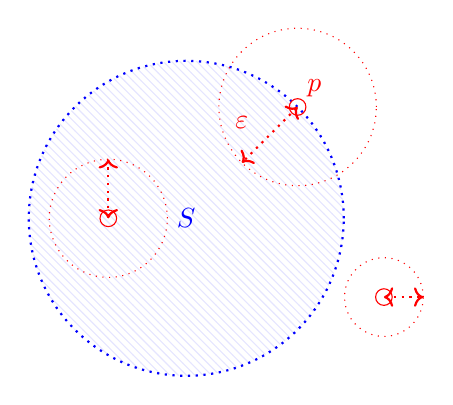
\begin{tikzpicture}[scale=1]
\fill[pattern=north west lines, pattern color=blue!10] (0,0) circle [radius=2];
\draw[dotted, thick, blue] (0,0) circle [radius=2] node[midway, blue] {$S$};

\draw[red] ({sqrt(2)}, {sqrt(2)}) circle (3pt) node[above right] {$p$};
\draw[dotted, red] ({sqrt(2)}, {sqrt(2)}) circle (1cm) node[below] {};
\draw[<->, dotted, thick, red] ({sqrt(2)}, {sqrt(2)}) to ({sqrt(1/2)},{sqrt(1/2)}) node[above=.3cm] {$\varepsilon$};

\draw[red] (-{.7*sqrt(2)}, 0) circle (3pt);
\draw[dotted, red] (-{.7*sqrt(2)}, 0) circle (.75cm);
\draw[<->, dotted, thick, red] (-{.7*sqrt(2)}, 0) to (-{.7*sqrt(2)}, .75);

\begin{scope}[shift={(3.5,-1)}]
	\draw[red] (-{.7*sqrt(2)}, 0) circle (3pt);
	\draw[dotted, red] (-{.7*sqrt(2)}, 0) circle (.5cm);
	\draw[<->, dotted, thick, red] (-{.7*sqrt(2)}, 0) to ({-.7*sqrt(2)+.5}, 0);
\end{scope}
\end{tikzpicture}
\end{center}
\begin{remark*}
	Note that a limit point $p$ may NOT belong to $S$.
\end{remark*}
{\color{gray!50}\begin{note}[Limit Point (Topology)]
	Let $(X,\tau)$ be a topological space. For a subset $S\subseteq X$. A point $p\in X$ is a limit point of $S$ if and only if \[
	\forall U\in\tau\ \text{with}\ p\in U,\ U\cap (S\setminus\set{p})\neq\varnothing.
	\]
\end{note}}
\begin{example*}
	Let $S=(a,b)\subseteq\R$:
	\begin{center}
	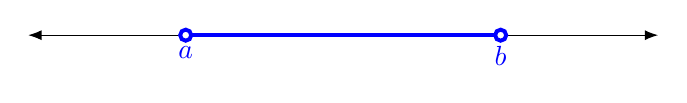
\begin{tikzpicture}
		\draw[Latex-Latex] (-4,0) to (4,0);
		\draw[line width=.5mm, blue] (-2,0) to (2,0);
		\draw[line width=.5mm, blue, fill=white] (-2,0) circle (2pt) node[below] {$a$};
		\draw[line width=.5mm, blue, fill=white] (2,0) circle (2pt) node[below] {$b$};
	\end{tikzpicture}
	\end{center}
\begin{itemize}
	\item[(i)] Consider $p$ with $p<a$:
	\begin{center}
	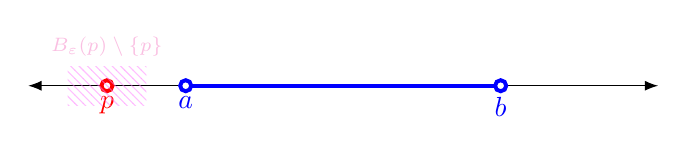
\begin{tikzpicture}
		\draw[Latex-Latex] (-4,0) to (4,0);
		\draw[line width=.5mm, blue] (-2,0) to (2,0);
		\draw[line width=.5mm, blue, fill=white] (-2,0) circle (2pt) node[below] {$a$};
		\draw[line width=.5mm, blue, fill=white] (2,0) circle (2pt) node[below] {$b$};
		\draw[line width=.5mm, red, fill=white] (-3,0) circle (2pt) node[below] {$p$};
		\fill[pattern=north west lines, pattern color=magenta!50, opacity=.5] (-3.5, -.25) rectangle (-2.5, 0.25);
		\node[above=.25cm, magenta!50, opacity=.5] at (-3,0) {\scriptsize $B_\varepsilon(p)\setminus\set{p}$};
%		\draw[decorate, decoration={brace, amplitude=5pt}, thick, color=magenta] (-3, .1) -- (-2.5, .1)
%		node[midway, above=5pt, color=magenta] {\( \varepsilon \)};
	\end{tikzpicture}
	\end{center}
	Let $\varepsilon:=\frac{a-p}{2}>0$. Then $B_\varepsilon(p)\cap (S\setminus\set{p})=\varnothing$. Thus, $p<a$ is NOT a limit point.
	\item[(ii)] Consider $p=a$:
	\begin{center}
	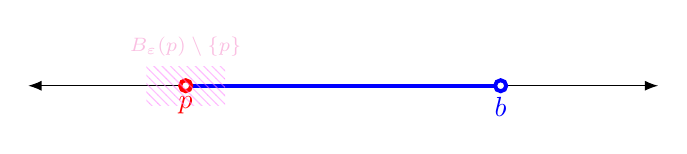
\begin{tikzpicture}
		\draw[Latex-Latex] (-4,0) to (4,0);
		\draw[line width=.5mm, blue] (-2,0) to (2,0);
%		\draw[line width=.5mm, blue, fill=white] (-2,0) circle (2pt) node[below] {$a$};
		\draw[line width=.5mm, blue, fill=white] (2,0) circle (2pt) node[below] {$b$};
		\draw[line width=.5mm, red, fill=white] (-2,0) circle (2pt) node[below] {$p$};
		\fill[pattern=north west lines, pattern color=magenta!50, opacity=.5] (-2.5, -.25) rectangle (-1.5, 0.25);
		\node[above=.25cm, magenta!50, opacity=.5] at (-2,0) {\scriptsize $B_\varepsilon(p)\setminus\set{p}$};
	\end{tikzpicture}
	\end{center}
	Let $\varepsilon>0$. Then $B_\varepsilon(p)\cap (S\setminus\set{p})\neq\varnothing$. Thus, $p=a$ is a limit point of $S=(a,b)$.
\end{itemize}
By (i) and (ii), the set of all limit points of $\intoo{a,b}$ is $\intcc{a,b}$.
\end{example*}
\vfill
\begin{example*}
	Let $S=\set{\frac{1}{n}:n\in\N}$:
	\begin{center}
	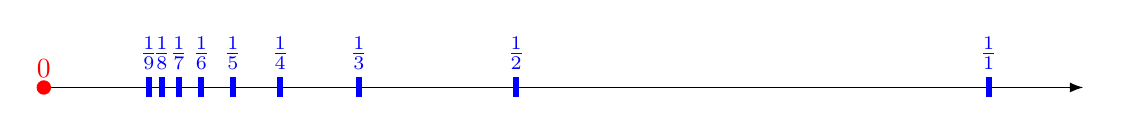
\begin{tikzpicture}[scale=12]
		\draw[-Latex] (0, 0) -- (1.1, 0) node[right] {};
		\foreach \n in {1, 2, 3, 4, 5, 6, 7, 8, 9} {
			%	\filldraw[blue] ({1/\n}, 0) circle (0.15pt) node[above] {$\frac{1}{\n}$};
			\filldraw[blue] ({1/\n-.0025},-.01) rectangle ({1/\n+.0025}, .01);
			\filldraw[blue] ({1/\n}, 0) circle (0) node[above=.1cm] {$\frac{1}{\n}$};
		}
		\filldraw[red] (0, 0) circle (0.2pt) node[above] {$0$};
	\end{tikzpicture}
	\end{center}
	\begin{itemize}
		\item Consider $p=\frac{1}{n}\in S$. No point of $S$ is a limit point.
		\item Consider $p=0$.
		\begin{center}
		\begin{tikzpicture}[scale=12]
			\draw[-Latex] (0, 0) -- (.5, 0) node[right] {};
			\filldraw[blue] ({1/9-.0025},-.01) rectangle ({1/9+.0025}, .01);
			\filldraw[blue] ({1/9}, 0) circle (0) node[above=.1cm] {$\frac{1}{n}$};
			\filldraw[magenta] ({1/5-.0025},-.015) rectangle ({1/5+.0025}, .015);
			\filldraw[magenta] ({1/5}, 0) circle (0) node[above=.15cm] {$\varepsilon$};
%			\foreach \n in {9} {
%				%	\filldraw[blue] ({1/\n}, 0) circle (0.15pt) node[above] {$\frac{1}{\n}$};
%				\filldraw[blue] ({1/\n-.0025},-.01) rectangle ({1/\n+.0025}, .01);
%				\filldraw[blue] ({1/\n}, 0) circle (0) node[above=.1cm] {$\frac{1}{n}$};
%			}
			\filldraw[red] (0, 0) circle (0.2pt) node[above] {$0$};
		\end{tikzpicture}
		\end{center}
		Let $\varepsilon>0$. By Archimedian property, $
		\exists n\in\N\ \text{such that}\ n>\frac{1}{\varepsilon},$ and so $1/n\in B_\varepsilon(0)\cap S$. Thus, $p=0$ is a limit point of $S=\set{1/n:n\in\N}$.
	\end{itemize}
\end{example*}

\newpage

\begin{example*}
Let $S=\Q$.
\begin{itemize}
	\item Consider $p\in\R$. Let $\varepsilon>0$. By density of rationals, \[
	\exists r\in\Q\ \text{such that}\ p<r<p+\varepsilon.
	\] Then $r\in B_\varepsilon(p)\cap S$ with $r\neq p$, \ie, $r$ is a limit points. Thus, all reals are limit points of $\Q$.
\end{itemize}
\end{example*}
%\begin{center}
%\begin{tikzpicture}[scale=3]
%	% Draw the coordinate axes
%%	\draw[->] (-2, 0) -- (4, 0) node[right] {x};
%%	\draw[->] (0, -2) -- (0, 4) node[above] {y};
%	% Define the set of points
%	\foreach \x/\y in {0.5/1, 1.5/0.5, 2/1.5, 2.5/2.2, 1.8/2.5, 1.2/2.3, 0.8/1.8} {
%		\fill[blue] (\x, \y) circle[radius=2pt];
%	}
%	% Highlight the limit point
%	\fill[red] (2, 1) circle[radius=2.5pt] node[below right] {$\alpha$};
%	% Draw the open ball
%	\draw[green!60!black, thick, dashed] (2, 1) circle (1);
%	\node[green!60!black] at (3, 2) {$B_\varepsilon(\alpha)$};
%	% Annotate nearby points in the open ball
%	\foreach \x/\y in {1.5/0.5, 2/1.5, 2.5/2.2} {
%		\draw[->, orange, thick] (\x, \y) -- (2, 1);
%	}
%	
%	% Explanation of other points
%	\node[blue] at (0.5, 0.5) {Other points in the set};
%	\node[red] at (2.8, 0.8) {Limit point $p$};
%\end{tikzpicture}
%\end{center}
\vfill
\defbox[$\star$ Limit of a Function ($\varepsilon-\delta$) $\star$]{\begin{definition*}
	Let $f:X\to\R$ be a function defined on a subset $X(\subseteq\R)$ of a metric space, and let $p\in X$ be a limit point of $X$. We say that $L\in\R$ is the \textbf{limit of the function $f$ as $x$ approaches $p$} if
	\[
	\boxed{\forall\varepsilon>0,\ \exists\delta>0\ \text{such that}\ \forall x\in X,\ 0<\abs[0]{x-p}<\delta\implies\abs[0]{f(x)-L}<\varepsilon}.
	\] We write \[
	\boxed{\lim\limits_{x\to p} f(x)=L}.
	\]
\end{definition*}}\vfill
\begin{center}
\begin{minipage}{.49\textwidth}
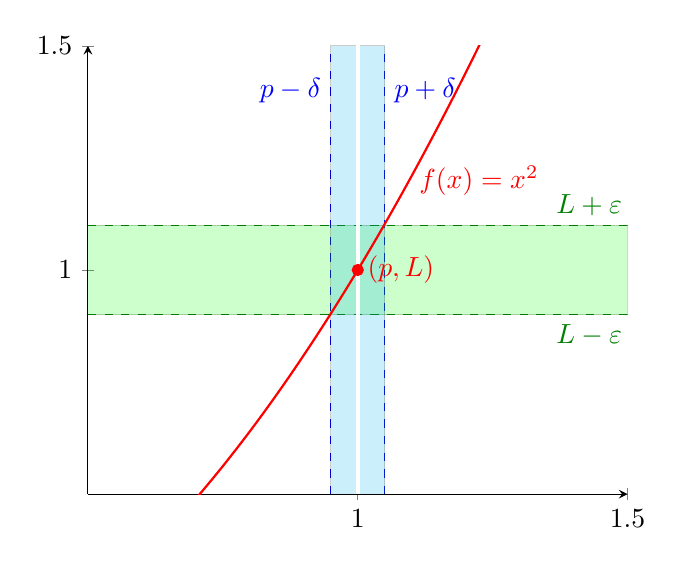
\begin{tikzpicture}
\begin{axis}[
axis lines=middle,
%xlabel={$x$},
%ylabel={$f(x)$},
xmin=0.5, xmax=1.5,
ymin=0.5, ymax=1.5,
xtick={0.5, 1, 1.5},
ytick={0.5, 1, 1.5},
xlabel style={below right},
ylabel style={above left},
legend pos=outer north east,
samples=100
]
% Horizontal epsilon bounds: L-eps and L+eps
\addplot[dashed, green!50!black] coordinates {(0.5, 0.9) (1.5, 0.9)} node[pos=0.85, below right] {$L - \varepsilon$};
\addplot[dashed, green!50!black] coordinates {(0.5, 1.1) (1.5, 1.1)} node[pos=0.85, above right] {$L + \varepsilon$};

% Vertical delta bounds: c-delta and c+delta
\addplot[dashed, blue] coordinates {(0.95, 0.5) (0.95, 1.5)} node[pos=0.9, left] {$p - \delta$};
\addplot[dashed, blue] coordinates {(1.05, 0.5) (1.05, 1.5)} node[pos=0.9, right] {$p + \delta$};

% Shaded area for epsilon bound
\addplot[fill=green, opacity=0.2] coordinates {
	(0.5, 0.9)
	(1.5, 0.9)
	(1.5, 1.1)
	(0.5, 1.1)
	(0.5, 0.9)
};

% Shaded area for delta bound
\addplot[fill=cyan, opacity=0.2] coordinates {
%	(0.9, 0.5)
	(1.05, 0.5)
	(1.05, 1.5)
	(0.95, 1.5)
	(0.95, 0.5)
};


% Shaded area for delta bound
\addplot[fill=white, draw=white] coordinates {
%	(0.9, 0.5)
	(1.0025, 0.5)
	(1.0025, 1.5)
	(0.9975, 1.5)
	(0.9975, 0.5)
};

% Function plot: f(x) = x^2
\addplot[domain=0.5:1.5, thick, red] {x^2} node[midway, right] {$f(x) = x^2$};
% Highlight point (c, L)
\addplot[only marks, mark=*, red] coordinates {(1, 1)} node[below, right] {$(p, L)$};
\end{axis}
\end{tikzpicture}
\end{minipage}\hfill
\begin{minipage}{.49\textwidth}
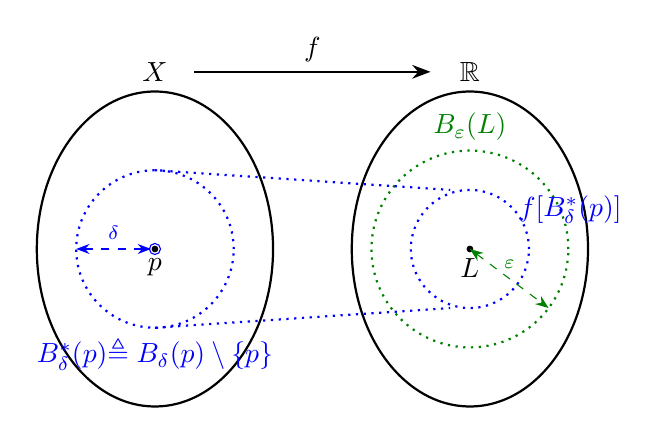
\begin{tikzpicture}[scale=1]
	\draw[thick] (-2,0) ellipse (1.5 and 2);
	\draw[blue, dotted, thick] (-2,0) ellipse (1 and 1);
	\node[below, blue,align=center] at (-2,-1) {$B_\delta^*(p)$$\triangleq B_\delta(p)\setminus\set{p}$};
	\draw[thick] (2,0) ellipse (1.5 and 2);
	\node[green!50!black, above] at (2,1.25) {$B_\varepsilon(L)$};
	\draw[green!50!black, dotted, thick] (2,0) ellipse (1.25 and 1.25);
	\draw[blue, dotted, thick] (2,0) ellipse (.75 and .75);
	\node[blue, right, align=left] at (2.5,.5) {$f[B_\delta^*(p)]$};
	
	% Labels for sets
	\node at (-2, 2.25) {$X$};
	\node at (2, 2.25) {$\R$};
	
	% Draw the arrows representing the function
	\draw[-Stealth, thick] (-1.5, 2.25) -- (1.5,2.25) node[midway, above] {$f$};
	
	%	\node at (2, 1.25) {$f[A]$};
	\draw[blue, dotted, thick] (-2, 1) -- (1.75, .75);
	\draw[blue, dotted, thick] (-2, -1) -- (1.75, -.75);
	
	\filldraw (-2,0) circle (1pt) node[below] {$p$};
	\draw[blue] (-2,0) circle (2pt);
	\filldraw (2,0) circle (1pt) node[below] {$L$};
	%	\draw[|->] (-1.85, 0) -- (1.85, 0);
	
	\draw[>=Stealth, <->, dashed, green!50!black] (2, 0) -- (3,-.75) node[midway, above] {\scriptsize $\varepsilon$};
	\draw[>=Stealth, <->, dashed, blue] (-2.05, 0) -- (-3,0) node[midway, above] {\scriptsize $\delta$};
\end{tikzpicture}
\end{minipage}
\end{center}
%\begin{center}
%\begin{tikzpicture}[scale=1.5]
%	\draw[thick] (-2,0) ellipse (1.5 and 2);
%	\draw[blue, dotted, thick] (-2,0) ellipse (1 and 1);
%	\node[above, blue] at (-2,1) {$B_\delta^*(p)\triangleq B_\delta(p)\setminus\set{p}$};
%	\draw[thick] (2,0) ellipse (1.5 and 2);
%	\node[red, above] at (2,1.25) {$B_\varepsilon(L)$};
%	\draw[red, dotted, thick] (2,0) ellipse (1.25 and 1.25);
%	\draw[blue, dotted, thick] (2,0) ellipse (.75 and .75);
%	\node[blue, right, align=left] at (2.5,.5) {$f[B_\delta^*(p)]$};
%	
%	% Labels for sets
%	\node at (-2, 2.25) {$X$};
%	\node at (2, 2.25) {$\R$};
%	
%	% Draw the arrows representing the function
%	\draw[-Stealth, thick] (-1.5, 2.25) -- (1.5,2.25) node[midway, above] {$f$};
%	
%	%	\node at (2, 1.25) {$f[A]$};
%	\draw[blue, dotted, thick] (-2, 1) -- (1.75, .75);
%	\draw[blue, dotted, thick] (-2, -1) -- (1.75, -.75);
%	
%	\filldraw (-2,0) circle (1pt) node[below] {$p$};
%	\draw[blue] (-2,0) circle (2pt);
%	\filldraw (2,0) circle (1pt) node[below] {$L$};
%%	\draw[|->] (-1.85, 0) -- (1.85, 0);
%	
%	\draw[>=Stealth, <->, dashed, red] (2, 0) -- (3,-.75) node[midway, above] {\scriptsize $\varepsilon$};
%	\draw[>=Stealth, <->, dashed, blue] (-2.05, 0) -- (-3,0) node[midway, above] {\scriptsize $\delta$};
%\end{tikzpicture}
%\end{center}
\vfill\begin{remark*}
\[
\lim\limits_{x\to p} f(x)\neq L\iff \exists\varepsilon>0:[\forall\delta>0:\exists x\in X: 0<\abs[0]{x-p}<\delta\ \text{but}\ \abs[0]{f(x)-L}>0].
\]
\end{remark*}
\defbox[Continuity of a Function]{\begin{definition*}
	Let $f:X\to\R$ be a function defined on a subset $X\subseteq\R$ of a metric space, and let $p\in X$. The function $f$ is \textbf{continuous at $p$} if and only if \[
	\lim\limits_{x\to p}f(x)=f(p).
	\] That is, \[
	\forall\varepsilon>0,\ \exists\delta>0\ \text{such that}\ \abs[0]{x-p}<\delta\implies\abs[0]{f(x)-f(p)}<\varepsilon.
	\]
\end{definition*}}
\begin{remark*}[Continuity of a Set]
	The function $f$ is continuous on subset $S\subseteq X$ if it is continuous at every point $p\in S$.
\end{remark*}

{\color{gray!50}\begin{remark*}[Continuity in a Topological Space]
	Let $(X,\tau_X)$ and $(Y,\tau_Y)$ are topological spaces. $f:X\to Y$ is \textbf{continuous} if and only if $$U_Y\in\tau_Y\implies f^{-1}[U_Y]\in\tau_X,$$ where $f^{-1}[U_Y]=\set{x\in X:f(x)\in U_Y}$ is the preimage of $U_Y$ under $f$.
\end{remark*}}
\vfill
\begin{note}
	$[p\Rightarrow(q\Rightarrow r)]\equiv [p\Rightarrow(\lnot q\lor r)]\equiv[\lnot p\lor (\lnot q\lor r)]\equiv [\lnot (p\land q)\lor r]\equiv [(p\land q)\Rightarrow r]$.
\end{note}
\thmbox[Limit of Function by Convergent Sequences]{\begin{theorem*}
Let $f:X\to\R$ be a function defined on a subset $\varnothing\neq X\subseteq\R$ of a metric space, and let $p$ is a limit point of $X$. Then \[
\lim\limits_{x\to p}f(x)=L\iff\left[\forall\set{x_n}\subseteq X\setminus\set{p},\left(\lim\limits_{n\to\infty}x_n=p\implies\lim\limits_{n\to\infty}f(x_n)=L\right)\right].
\]
\end{theorem*}}
\begin{center}
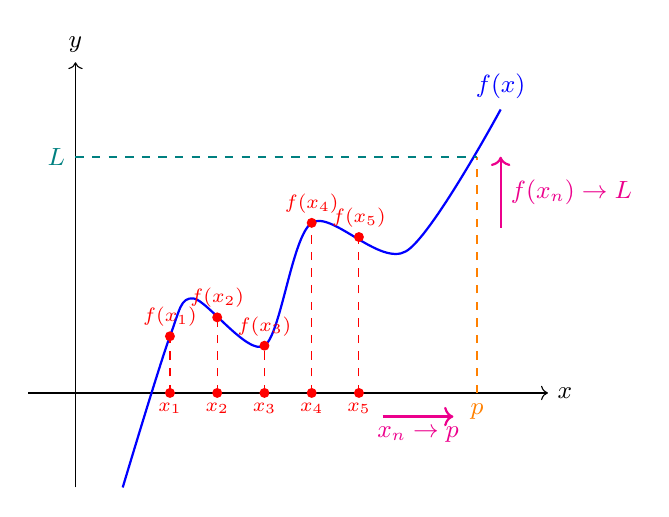
\begin{tikzpicture}[scale=1.2, every node/.style={font=\small}]
	% Axes
	\draw[->] (-0.5, 0) -- (5, 0) node[right] {$x$};
	\draw[->] (0, -1) -- (0, 3.5) node[above] {$y$};
	
	\begin{scope}[shift={(-.5,3)}]
		\draw[color=blue,thick,smooth] plot coordinates {(1,-4) (1.5,-2.4) (1.75,-2) (2.5,-2.5) (3,-1.2) (4,-1.5) (5,0)} node[above] {$f(x)$};
	\end{scope}
	
	% Points and labels for the sequence x_n
	\foreach \n/\x/\y in {1/1/.6, 2/1.5/.8, 3/2/.5, 4/2.5/1.8, 5/3/1.65}
	{
		\fill[red] (\x, \y) circle (1.5pt) node[above] {\scriptsize $f(x_{\n})$};
		\fill[red] (\x, 0) circle (1.5pt) node[below] {\scriptsize $x_{\n}$};
		\draw[red, dashed] (\x, 0) -- (\x, \y);
	}

	% Converging sequence x_n -> a
	\draw[magenta, ->, thick] (3.25, -0.25) -- (4, -0.25) node[midway, below] {$x_n \to p$};
	
	% Converging sequence f(x_n) -> L
	\draw[magenta, ->, thick] (4.5, 1.75) -- (4.5, 2.5) node[midway, right] {$f(x_n) \to L$};
	
	% Labels for a and L
	\draw[dashed, thick, orange] (4.25, 0) node[below] {$p$} -- (4.25, 2.5);
	\draw[dashed, thick, teal] (0, 2.5) node[left] {$L$} -- (4.25, 2.5);
	
\end{tikzpicture}
\end{center}
%\begin{tikzpicture}[scale=1.5]
%	% Axes
%	\draw[->] (-1, 0) -- (5, 0) node[right] {\(x\)};
%	\draw[->] (0, -1) -- (0, 4) node[above] {\(y\)};
%	
%	% Function curve
%	\draw[domain=0.5:4, smooth, variable=\x, thick] plot ({\x}, {2 + 0.5*sin(3*\x r)});
%	\node[below right] at (4, 3) {\(f(x)\)};
%	
%	% Limit point
%	\node[below] at (2, 0) {\(p\)};
%	\node[left] at (0, 2.5) {\(L\)};
%	\draw[dashed] (2, 0) -- (2, 2.5);
%	\draw[dashed] (0, 2.5) -- (2, 2.5);
%	
%	% Sequence points
%	\foreach \i in {1, 2, 3, 4} {
%		\pgfmathsetmacro{\xn}{2 - 1/\i}
%		\pgfmathsetmacro{\yn}{2.5 + 0.5*sin(3*\xn r)}
%		\draw[fill=blue] (\xn, \yn) circle (1pt);
%		\draw[dashed, blue] (\xn, \yn) -- (\xn, 0);
%		\node[below] at (\xn, 0) {\(x_{\i}\)};
%	}
%	
%	% Sequence convergence
%	\draw[->, thick, red] (1.2, 3.5) -- (2, 2.5) node[above left] {\(f(x_n) \to L\)};
%\end{tikzpicture}
\begin{proof}
\begin{itemize}
	\item[($\Rightarrow$)] Suppose that $\lim\limits_{x\to p}f(x)=L$. Let $\set{x_n}\subseteq X\setminus\set{p}$ be a sequence, and let $\lim\limits_{n\to\infty}x_n=p$. We NTS that \[
	\lim\limits_{n\to\infty}f(x_n)=L,\quad\ie,\color{blue}\quad\forall\varepsilon>0:\exists N\in\N:n\geq N\Rightarrow\abs[0]{f(x_n)-L}<\varepsilon.
	\] \textcolor{blue}{Let $\varepsilon>0$}. Since $\lim\limits_{x\to p}f(x)=L$, we know \begin{equation*}
		\exists\delta>0\ \text{such that}\ 0<\abs[0]{x-p}<\delta\implies\abs[0]{f(x)-L}<\varepsilon.\tag{*}
	\end{equation*} Since $\lim\limits_{n\to\infty}x_n=p$, we obtain \[
	\textcolor{blue}{\exists N\in\N}\ \text{such that}\ n\geq N\implies\abs[0]{x_n-p}<\delta.
	\] Thus, \textcolor{blue}{if $n\geq N$ then}, \begin{align*}
		\abs[0]{x_n-p}<\delta&\implies 0<\abs[0]{x_n-p}<\delta\quad\because x_n\neq p \\
		&\implies\textcolor{blue}{\abs[0]{f(x_n)-L}<\varepsilon}\quad\text{by (*)}
	\end{align*} Thus, $\lim\limits_{n\to\infty}f(x_n)=L$.
	\item[($\Leftarrow$)] Let the RHS holds. Assume, for the contradiction, that $\lim\limits_{x\to p} f(x)\neq L$, \ie, \[
	\textcolor{green!50!black}{\exists\varepsilon>0}:\forall\delta>0:\exists x_\delta\in X:0<\abs[0]{x_\delta-p}<\delta\ \text{but}\ \textcolor{magenta}{\abs[0]{f(x_\delta)-L}\geq\varepsilon}.
	\] Take $\delta=1/n$ for $n\in\N$. Then \[
	\exists x_n\in X\ \text{such that}\ 0<\abs[0]{x_n-p}<\frac{1}{n}\ \text{but}\ \abs[0]{f(x_n)-L}\geq \varepsilon.
	\] \textcolor{gray!50}{\st{(Axiom of Countable Choice)}}\ This means that \[
	\forall n\in\N:\exists\set{x_n}\subseteq X\setminus\set{p}\ \text{such that}\ 0<\abs[0]{x_n-p}<\frac{1}{n}\ \text{but}\ \textcolor{magenta}{\abs[0]{f(x_n)-L}\geq \varepsilon}.
	\] By Squeeze Theorem, we have $\lim\limits_{n\to\infty}x_n=p$ since $0<\abs[0]{x_n-p}<1/n$. Since the RHS holds, we obtain $\lim\limits_{n\to\infty}f(x_n)=L$. Then, for some $\textcolor{green!50!black}{\varepsilon>0}$, \[
	\exists N\in\N\ \text{such that}\ n\geq N\implies\textcolor{magenta}{\abs{f(x_n)-L}<\varepsilon}\ \text{\Large\lightning}.
	\] Hence it is proved.
\end{itemize}
\end{proof}
\corbox[Continuity of Function by Convergent Sequences]{\begin{corollary*}
Let $f:X\to\R$ be a function defined on a subset $\varnothing\neq X\subseteq\R$ of a metric space, and let $p$ is a limit point of $X$. Then \[
\lim\limits_{x\to p}f(x)=f(p)\iff\left[\forall\set{x_n}\subseteq X,\left(\lim\limits_{n\to\infty}x_n=p\implies\lim\limits_{n\to\infty}f(x_n)=f(p)\right)\right].
\]
\end{corollary*}}
\vfill
\thmbox[Squeeze Theorem; Sandwich Theorem]{\begin{theorem*}
	Let \begin{enumerate}[(i)]
		\item $\lim\limits_{n\to\infty}a_n=L=\lim\limits_{n\to\infty}b_n$;
		\item $\exists n_0\in\N$ such that $a_n\leq c_n\leq b_n$ for all $n\geq n_0$.
	\end{enumerate} Then $
	\lim\limits_{n\to\infty}c_n=L.$
\end{theorem*}}
\begin{center}
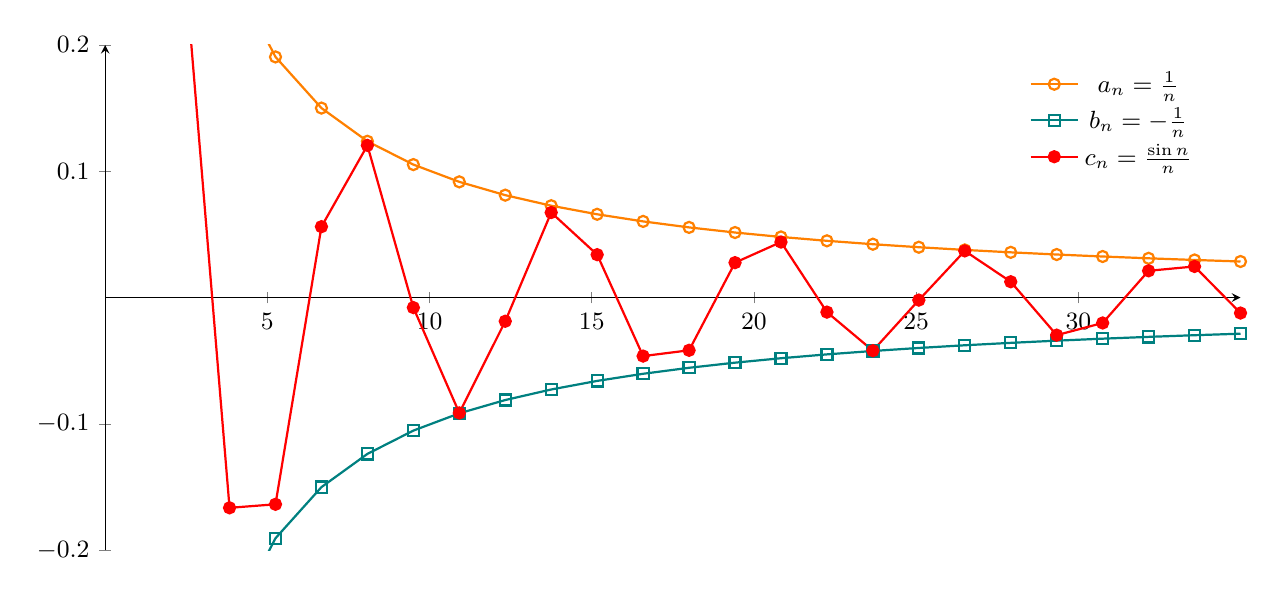
\begin{tikzpicture}
	\begin{axis}[
		width=16cm, height=8cm, % Size of the plot
		axis lines=middle,
%		xlabel={$n$},
%		ylabel={$a_n, b_n, c_n$},
		xmin=0, xmax=35, % n range
		ymin=-0.2, ymax=0.2, % y range
		xtick={0,5,10,15,20,25,30}, % n ticks
		ytick={-0.2,-0.1,0,0.1,0.2}, % y ticks
		legend style={draw=none, fill=none, font=\small},
		legend pos=north east,
		every axis x label/.style={at={(current axis.right of origin)}, anchor=north},
		every axis y label/.style={at={(current axis.above origin)}, anchor=east},
		tick label style={font=\small}
		]
		
		% Plot a_n = 1/n
		\addplot[domain=1:35, thick, orange, mark=o] {1/x};
		\addlegendentry{$a_n = \frac{1}{n}$}
		
		% Plot b_n = -1/n
		\addplot[domain=1:35, thick, teal, mark=square] {-(1/x)};
		\addlegendentry{$b_n = -\frac{1}{n}$}
		
		% Plot c_n = sin(n)/n
		\addplot[domain=1:35, thick, red, mark=*] {sin(deg(x))/x};
		\addlegendentry{$c_n = \frac{\sin n}{n}$}
	\end{axis}
\end{tikzpicture}
\end{center}
\begin{proof}
\textcolor{blue}{Let $\varepsilon>0$}. Since $\lim\limits_{n\to\infty}a_n=L$ and $\lim\limits_{n\to\infty}a_n=L$, we have \begin{align*}
\exists n_1\in\N\ \text{such that}\ n\geq n_1&\implies L-\varepsilon<a_n\textcolor{gray}{<L+\varepsilon},\\
\exists n_2\in\N\ \text{such that}\ n\geq n_2&\implies \textcolor{gray}{L-\varepsilon}<b_n<L+\varepsilon.
\end{align*} Let \textcolor{blue}{$N:=\max\set{n_0,n_1,n_2}$}. \textcolor{blue}{If $n\geq N$ then} \[
L-\varepsilon<a_n\leq c_n\leq b_n<L_+\varepsilon,
\] and so \textcolor{blue}{$\abs[0]{c_n-L}<\varepsilon$}.
\end{proof}
%\newpage
%\begin{example*} Prove that \[
%\lim\limits_{n\to\infty}n^{\frac{1}{n}} = 1.	
%\]
%\begin{center}
%\begin{tikzpicture}
%\begin{axis}[
%	width=12cm, height=8cm, % Plot size
%	axis lines=middle,
%%	xlabel={$n$},
%%	ylabel={$a_n = n^{1/n}$},
%	xmin=1, xmax=30, % Set x-axis range
%	ymin=0.9, ymax=1.5, % Set y-axis range
%	xtick={0,5,10,15,20,25,30}, % Custom x-ticks
%	ytick={0.9,1,1.1,1.2}, % Custom y-ticks
%	legend style={draw=none, fill=none, font=\small},
%	legend pos=north east,
%	every axis x label/.style={at={(current axis.right of origin)}, anchor=south},
%	every axis y label/.style={at={(current axis.above origin)}, anchor=west},
%	tick label style={font=\small}
%	]
%	% Plot a_n = n^(1/n)
%	\addplot[domain=1:30, thick, blue, mark=*] {x^(1/x)};
%	\addlegendentry{$x_n = n^{1/n}$}
%	
%	% Plot y = 1 (limit line)
%	\addplot[dashed, red] coordinates {(1,1) (30,1)};
%	\addlegendentry{$L = 1$}
%\end{axis}
%\end{tikzpicture}
%\end{center}
%\begin{proof}[\sol]
%	Let $x_n=n^{1/n}$ and $x_n=1+a_n$. Then
%\end{proof}
%\begin{tikzpicture}
%\ \\	\begin{axis}[
%		width=12cm, height=8cm, % Set plot size
%		axis lines=middle,
%		xlabel={$n$},
%		ylabel={$a_n, b_n$},
%		xmin=1, xmax=20, % Set x-axis range
%		ymin=-2, ymax=2, % Set y-axis range
%		xtick={1,5,10,15,20}, % Custom x-ticks
%		ytick={0.9,1,1.1,1.2}, % Custom y-ticks
%		legend style={draw=none, fill=none, font=\small},
%		legend pos=south east,
%		every axis x label/.style={at={(current axis.right of origin)}, anchor=north},
%		every axis y label/.style={at={(current axis.above origin)}, anchor=east},
%		tick label style={font=\small}
%		]
%		% Plot b_n = sqrt(2/(n-1))
%		\addplot[domain=2:20, thick, red, mark=o] {sqrt(2/(x-1))};
%		\addlegendentry{$b_n = \sqrt{\frac{2}{n-1}}$}
%		
%		% Plot a_n = 1 + b_n
%		\addplot[domain=2:20, thick, blue, mark=*] {1 + sqrt(2/(x-1))};
%		\addlegendentry{$a_n = 1 + b_n$}
%		
%		% Plot y = 1 (limit line for a_n)
%		\addplot[dashed, black] coordinates {(1,1) (20,1)};
%		\addlegendentry{$L = 1$}
%		
%		% Annotate
%		\node[anchor=south] at (axis cs:15,1.15) {As $n \to \infty, \ b_n \to 0$ and $a_n \to 1$};
%	\end{axis}
%\end{tikzpicture}
%\end{example*}

\newpage
\begin{note}
	Recall that
	\begin{center}
		``A convergent sequence is bounded.''
	\end{center}
Formally, \[
\exists A\in\R\ \text{s.t.}\ A=\lim_{n\to\infty}a_n\implies\exists M\in\R\ \text{s.t.}\ \forall n\in\N,\ \abs{a_n}\leq M.
\]However, the converse is not necessarily true: \[
\exists A\in\R\ \text{s.t.}\ A=\lim_{n\to\infty}a_n\centernot\impliedby\exists M\in\R\ \text{s.t.}\ \forall n\in\N,\ \abs{a_n}\leq M.
\] To illustrate, consider the sequence \(\{a_n\} = 1 - (-1)^n\) that is bounded, yet it does not converge.
\vfill
\defbox[Monotone Sequence]{\begin{definition*}
	A sequence $\set{a_n}_{n=1}^\infty$ is said to be \textbf{monotone} if it is either \textbf{monotone increasing} or \textbf{monotone decreasing}.
	\begin{enumerate}[(1)]
		\item A sequence $\set{a_n}_{n=1}^\infty$ is \textbf{monotone increasing} if $
		a_n\leq a_{n+1}$ for all $n\in\N$.\par Alternatively, it is \textbf{strictly increasing} if $a_n<a_{n+1}$ for all $n\in\N$.
		\item A sequence $\set{a_n}_{n=1}^\infty$ is \textbf{monotone decreasing} if $
		a_{n+1}\leq a_{n}$ for all $n\in\N$.\par Alternatively, it is \textbf{strictly decreasing} if $a_{n+1}<a_{n}$ for all $n\in\N$.
	\end{enumerate}
\end{definition*}}
\begin{remark*}
A sequence $\set{a_n}$ is monotone if $\begin{cases*}
	a_n\leq a_{n+1} & (monotone increasing) \\
	a_{n+1}\leq a_n & (monotone decreasing)
\end{cases*}$.
\end{remark*}
\begin{example*}
\ \begin{itemize}
	\item $\set{n}_{n=1}^\infty$ is monotone increasing.
	\item $\set{1/n}_{n=1}^\infty$ is monotone decreasing.
\end{itemize}
\end{example*}
\begin{example*}
Let $0<x<1$.\\ \adjustbox{scale=1,center}{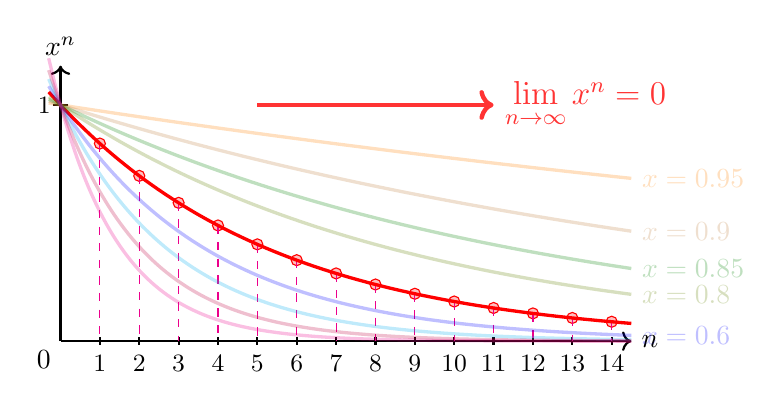
\begin{tikzpicture}[scale=1]
	% Axes
	\draw[->,thick] (0,0) -- (7.25,0) node[right] {$n$};
	\draw[->,thick] (0,0) -- (0,3.5) node[above] {$x^n$};
	
	% Ticks and labels for x-axis
	\foreach \x [count=\n from 1] in {.5,1,...,7} {
		\draw[thick] (\x,0.05) -- (\x,-0.05) node[below] {\small $\n$};
	}

	% Ticks and labels for y-axis
	\foreach \y in {3} {
		\draw[thick] (0.1,\y) -- (-0.1,\y);
		\ifnum\y=3
		\node[left] at (0,\y) {\small 1};
		\fi
	}
	
	% Sequence points for x = 0.8
	\foreach \n in {.5,1,...,7} {
		\pgfmathsetmacro{\yn}{0.7^\n}
		\draw[fill=pink,draw=red] (\n,3*\yn) circle (2pt);
		\draw[dashed,magenta] (\n,3*\yn) -- (\n,0);
	}
	
	% Convergence arrow and explanation
	\draw[->,ultra thick,red!80] (2.5,3) -- (5.5,3) node[right] {\large\textcolor{red!80}{$\lim\limits_{n \to \infty} x^n = 0$}};
	
	% Additional visual enhancement for the curve
	\draw[very thick,red,smooth] plot[domain=-.15:7.25,samples=100] (\x,{3*0.7^(\x)});
	\draw[very thick,orange, smooth, opacity=0.25] plot[domain=-.15:7.25,samples=100] (\x,{3*0.95^(\x)}) node[right] {$x=0.95$};
	\draw[very thick,brown, smooth, opacity=0.25] plot[domain=-.15:7.25,samples=100] (\x,{3*0.9^(\x)}) node[right] {$x=0.9$};
	\draw[very thick,green!50!black, smooth, opacity=0.25] plot[domain=-.15:7.25,samples=100] (\x,{3*0.85^(\x)}) node[right] {$x=0.85$};
	\draw[very thick,lime!50!black, smooth, opacity=0.25] plot[domain=-.15:7.25,samples=100] (\x,{3*0.8^(\x)}) node[right] {$x=0.8$};
	\draw[very thick,blue, smooth, opacity=0.25] plot[domain=-.15:7.25,samples=100] (\x,{3*0.6^(\x)}) node[right] {$x=0.6$};
	\draw[very thick,cyan, smooth, opacity=0.25] plot[domain=-.15:7.25,samples=100] (\x,{3*0.5^(\x)});
	\draw[very thick,purple, smooth, opacity=0.25] plot[domain=-.15:7.25,samples=100] (\x,{3*0.4^(\x)});
	\draw[very thick,magenta, smooth, opacity=0.25] plot[domain=-.15:7.25,samples=100] (\x,{3*0.3^(\x)});
	
%	\node[below right,blue!70!black] at (3.5,0.25) {\textbf{Illustration for} $x = 0.8$};
	
	% Labels and additional details
	\node[below left] at (0,0) {0};
%	\node[right,align=left] at (1,0.8) {\textbf{Monotone\ Convergence}};
%	\node[align=left,right] at (1.5,4.75) {\textit{The sequence $x^n$ is monotone\ and converges to zero.}};
\end{tikzpicture}}
\end{example*}
\newpage
\end{note}
\thmbox[Monotone Convergence Theorem (MCT)]{\begin{theorem*}\hypertarget{mct}{}
A monotone sequence of real numbers $\set{a_n}$ is convergent if and only if it is bounded.
\begin{enumerate}[(1)]
	\item Let $\set{a_n}$ be an \underline{monotone increasing} sequence of real numbers that is \underline{bounded above}. Then \[
	\lim\limits_{n\to\infty}a_n=\sup\set{a_n:n\in\N}.
	\]
	\item Let $\set{b_n}$ be an \underline{monotone decreasing} sequence of real numbers that is \underline{bounded below}. Then \[
	\lim\limits_{n\to\infty}b_n=\inf\set{b_n:n\in\N}.
	\]
\end{enumerate}
\end{theorem*}}
\begin{proof}
\ \begin{enumerate}[(1)]
	\item Suppose that a sequence $\set{a_n}$ is monotone increasing and bounded above. Consider the set $\set{a_n:n\in\N}\subseteq\R$, which is non-empty and bounded above by assumption. By \textbf{Least Upper Bound Property}\footnote{Every non-empty subset of $\R$ that is bounded above has the supremum in $\R$.}, \[
	\exists\alpha\in\R\ \text{such that}\ \alpha=\sup\set{a_n:n\in\N}.
	\] We claim that: \[
	\lim\limits_{n\to\infty}a_n=\alpha=\sup\set{a_n:n\in\N}.
	\] \textcolor{blue}{Let $\varepsilon>0$}. Since $\alpha$ is the supremum (\textit{least} upper bound) of $\set{a_n:n\in\N}$,  it follows that $\alpha-\varepsilon$ is not an upper bound of $\set{a_n:n\in\N}$. Thus, $\lnot[\forall N\in\N,\ a_N\leq\alpha-\varepsilon]$, \ie, \[
	\textcolor{blue}{\exists N\in\N}\ \text{such that}\ \alpha-\varepsilon<a_N.
	\] Since $\set{a_n}$ is monotone increasing, \[
	\alpha-\varepsilon<a_N\leq a_n
	\] for all $n\geq N$. Therefore, \[
	\alpha-\varepsilon\overset{\alpha=\sup\set{a_n}}{\underset{\varepsilon>0}{<}}a_N
	\overset{\set{a_n}\ \text{is monotone increasing}}{\underset{n\geq N}{\leq}}a_n\overset{\alpha\ \text{is an upper bound}}{\leq}\alpha\overset{\varepsilon>0}{<}\alpha+\varepsilon.
	\] This implies that \textcolor{blue}{$\abs[0]{a_n-\alpha}<\varepsilon$ for all $n\geq N$}.
	\newpage
	\item Suppose that a sequence $\set{b_n}$ is monotone decreasing and bounded below. Consider the set $\set{b_n:n\in\N}\subseteq\R$, which is non-empty and bounded below by assumption. By \textbf{Greatest Lower Bound Property}\footnote{Every non-empty subset of $\R$ that is bounded below has the infimum in $\R$.}, \[
	\exists\beta\in\R\ \text{such that}\ \beta=\inf\set{b_n:n\in\N}.
	\] We claim that: \[
	\lim\limits_{n\to\infty}b_n=\beta=\inf\set{b_n:n\in\N}.
	\] \textcolor{blue}{Let $\varepsilon>0$}. Since $\beta$ is the infimum (\textit{greatest} lower bound) of $\set{b_n:n\in\N}$,  it follows that $\beta+\varepsilon$ is not a lower bound of $\set{b_n:n\in\N}$. Thus, $\lnot[\forall N\in\N,\ \beta+\varepsilon\leq b_N]$, \ie, \[
	\textcolor{blue}{\exists N\in\N}\ \text{such that}\ b_N<\beta+\varepsilon.
	\] Since $\set{b_n}$ is monotone decreasing, \[
	b_n\leq b_N<\beta+\varepsilon
	\] for all $n\geq N$. Therefore, \[
	\beta-\varepsilon\overset{\varepsilon>0}{<}\beta\overset{\beta\ \text{is a lower bound}}{\leq}b_n\overset{\set{b_n}\ \text{is monotone decreasing}}{\underset{n\geq N}{\leq}} b_N\overset{\beta=\inf\set{b_n}}{\underset{\varepsilon>0}{<}}\beta+\varepsilon
	\]
	This implies that \textcolor{blue}{$\abs[0]{b_n-\beta}<\varepsilon$ for all $n\geq N$}.
\end{enumerate}
\end{proof}

\defbox[Divergence of Sequence]{\begin{definition*}
	Let $\set{a_n}$ be a sequence of real numbers. \begin{enumerate}[(1)]
		\item We say that the sequence $\set{a_n}$ \textbf{diverges to infinity} (or \textbf{tends to infinity}) if \[
		\forall M\in\R,\ \exists N\in\N\ \text{such that}\ n\geq N\implies M < a_n,
		\] and write $\lim\limits_{n\to\infty}a_n=+\infty.$
		\item We say that the sequence $\set{a_n}$ \textbf{diverges to minus infinity} (or \textbf{tends to infinity}) if \[
		\forall M\in\R,\ \exists N\in\N\ \text{such that}\ n\geq N\implies a_n < M,
		\] and write $\lim\limits_{n\to\infty}a_n=-\infty.$
		\item[\color{gray!50} (3)] 
		\text{\color{gray!50} We say that $\set{a_n}$ is properly divergent in case we have either $\lim\limits_{n\to\infty}a_n=+\infty$ or $\lim\limits_{n\to\infty}=-\infty$.}
	\end{enumerate}
\end{definition*}}
\begin{note}
	Recall that \begin{enumerate}[]
	\item \textbf{(Monotonicity)} A sequence $\set{a_n}$ is monotone increasing if $a_n\leq a_{n+1}$ for all $n\in\N$;
	\item \textbf{(Not Bounded Above)} The sequence $\set{a_n}$ is not bounded above if \[
	\lnot[\exists M\in\R,\ \forall n\in\N,\ a_n\leq M]\equiv [\forall M\in\R,\ \exists n\in\N\ \text{such that}\ a_n>M].
	\] We claim that a sequence $\set{a_n}$ that is monotone increasing and not bounded above diverges to infinity:\par
	\begin{proof}
		\textcolor{blue}{Let $M\in\R$}. Since $\set{a_n}$ is not bounded above, \[
		\textcolor{blue}{\exists n_0\in\N}\ \text{such that}\ a_{n_0}>M.
		\] Since $\set{a_n}$ is monotonic increasing, it fllows that \[
		a_{n_0}\leq a_n,\ \forall n\geq n_0.
		\] Thus \[
		\textcolor{blue}{n\geq n_0}\overset{\text{monotone increasing}}{\implies} a_{n_0}\leq a_n\overset{\text{Not Bounded Above}}{\textcolor{blue}{\implies}}\textcolor{blue}{M}<a_{n_0}\textcolor{blue}{<a_n}.
		\] Hence it is proved.
	\end{proof}
\end{enumerate}
Note that
\end{note}

\newpage
\lembox[]{\begin{lemma*}
		Let $\set{a_n}$ and $\set{b_n}$ be sequences of real numbers. Then \[
		\left[\forall n\in\N,\ a_n\leq b_n\right]\implies\lim\limits_{n\to\infty}a_n\leq \lim\limits_{n\to\infty}b_n.
		\] 
\end{lemma*}}
\begin{proof}
	Let $a=\lim\limits_{n\to\infty}a_n$ and $b=\lim\limits_{n\to\infty}b_n$. Suppose that $a>b$. Let $\varepsilon=a-b>0$. Then \begin{align*}
		\exists N_1\in\N\ \text{such that}\ &n\geq N_1\implies\abs{a_n-a}<\varepsilon,\\
		\exists N_2\in\N\ \text{such that}\ &n\geq N_2\implies\abs{b_n-b}<\varepsilon.
	\end{align*} Let $N:=\max\set{N_1,N_2}$. Then $b_N<b+\varepsilon<a+\varepsilon<a_N$\ \text{\Large\lightning}. Hence $a\leq b$, \ie, $\lim\limits_{n\to\infty}a_n\leq\lim\limits_{n\to\infty} b_n$.
\end{proof}
\vfill
\begin{note}
Let $I_n=\intoo{0,\frac{1}{n}}\subseteq\R$ for all $n\in\N$.
\begin{center}
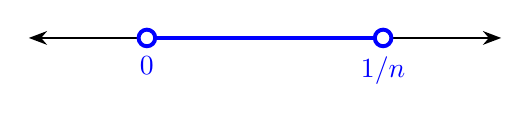
\begin{tikzpicture}[scale=1.5]
\draw[thick, Stealth-Stealth] (0, 0) -- (4, 0);
\draw[line width=.5mm, blue] (1, 0) -- (3, 0);
\draw[line width=.5mm, fill=white, draw=blue] (1,0) circle (2pt) node[blue, below, yshift=-.1cm] {$0$};
\draw[line width=.5mm, fill=white, draw=blue] (3,0) circle (2pt) node[blue, below, yshift=-.1cm] {$1/n$};
\end{tikzpicture}
\end{center}
Suppose that $x\in\bigcap_{n=1}^\infty I_n$ then $x\in I_n$ for all $n\geq 1$. That is, \[
0< x<\frac{1}{n}\quad\text{for all}\quad n\geq 1.
\] By Archimedian property, $\exists n_0\in\N$ s.t. $n_0x > 1$\ \text{\Large\lightning}. Hence $\bigcap_{n=1}^\infty I_n=\varnothing$.
\end{note}
\vfill
\begin{note}
Let $I_n=\intco{n,\infty}\subseteq\R$ for all $n\in\N$.
\begin{center}
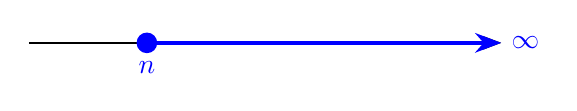
\begin{tikzpicture}[scale=1.5]
	\draw[thick, -Stealth] (0, 0) -- (4, 0) node[right, blue] {$\infty$};
	\draw[line width=.5mm, blue, -Stealth] (1, 0) -- (4, 0);
	\draw[line width=.5mm, fill=blue, draw=blue] (1,0) circle (2pt) node[blue, below, yshift=-.1cm] {$n$};
\end{tikzpicture}
\end{center}
Suppose that $x\in\bigcap_{n=1}^\infty I_n$ then $x\in I_n$ for all $n\geq 1$. That is, \[
n\leq x\quad\text{for all}\quad n\geq 1.
\] By Archimedian property, $\exists n_0\in\N$ s.t. $x < n_0$\ \text{\Large\lightning}. Hence $\bigcap_{n=1}^\infty I_n=\varnothing$.
\end{note}
\newpage
\thmbox[Nested Interval Property (NIP)]{\begin{theorem*}\hypertarget{nip}{}
	Let $a_n\leq b_n$ for all $n\in\N$, and let $\set{\intcc{a_n,b_n}}_{i=1}^\infty\subseteq\R$​
	be a sequence of bounded and closed intervals satisfying $\intcc{a_{n+1},b_{n+1}}\subseteq \intcc{a_n,b_n}$ for all $n\in\N$. Then \[
	\bigcap_{n=1}^\infty\intcc{a_n,b_n}:=\set{x\in\R: x\in\intcc{a_n,b_n}\ \text{for all}\ n\in\N}\neq\varnothing.
	\] 
%	In other word, $\exists x\in\R$ such that $x\in\intcc{a_n,b_n}$ for all $n\in\N$.
\end{theorem*}
\tcblower
If $\lim\limits_{n\to\infty}(b_n-a_n)=0$, then $\abs{\bigcap_{n=1}^\infty\intcc{a_n,b_n}}=1$.}
\begin{center}
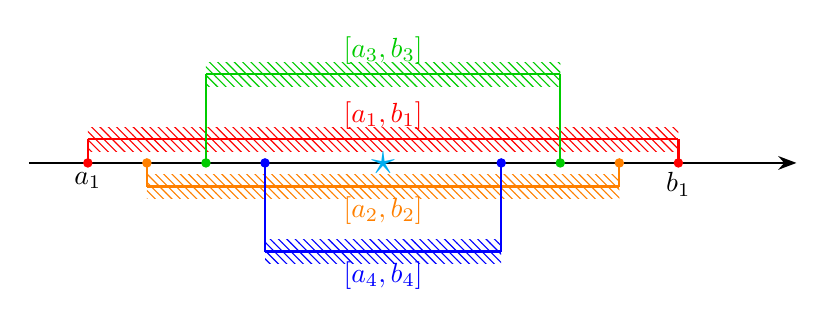
\begin{tikzpicture}[scale=1.5]
	
	% Draw the number line
	\draw[thick, -Stealth] (-0.5, 0) -- (6, 0);
	
	% Labels for endpoints
	\node[below] at (0, 0) {$a_1$};
	\node[below] at (5, 0) {$b_1$};
	
	% First interval
	\fill[pattern=north west lines, pattern color=red] (0, 0.1) rectangle (5, 0.3);
	\draw[red, thick] (0, 0.2) -- (5, 0.2);
	\draw[red, thick] (0, 0.2) -- (0, 0);
	\draw[red, thick] (5, 0.2) -- (5, 0);
	\node[red, above] at (2.5, 0.2) {$[a_1, b_1]$};
	\filldraw[red] (5,0) circle (1pt);
	\filldraw[red] (0,0) circle (1pt);
	
	% Second interval
	\fill[pattern=north west lines, pattern color=orange] (.5, -.1) rectangle (4.5, -0.3);
	\draw[orange, thick] (0.5, -0.2) -- (4.5, -0.2);
	\draw[orange, thick] (0.5, -0.2) -- (0.5, 0);
	\draw[orange, thick] (4.5, -0.2) -- (4.5, 0);
	\node[orange, below] at (2.5, -0.2) {$[a_2, b_2]$};
	\filldraw[orange] (4.5,0) circle (1pt);
	\filldraw[orange] (0.5,0) circle (1pt);
	
	% Third interval
	\fill[pattern=north west lines, pattern color=green!80!black] (1, .65) rectangle (4, .85);
	\draw[green!80!black, thick] (1, .75) -- (4, .75);
	\draw[green!80!black, thick] (1, .75) -- (1, 0);
	\draw[green!80!black, thick] (4, .75) -- (4, 0);
	\node[green!80!black, above] at (2.5, .75) {$[a_3, b_3]$};
	\filldraw[green!80!black] (4,0) circle (1pt);
	\filldraw[green!80!black] (1,0) circle (1pt);
	
	% Fourth interval
	\fill[pattern=north west lines, pattern color=blue] (1.5, -.65) rectangle (3.5, -.85);
	\draw[blue, thick] (1.5, -.75) -- (3.5, -.75);
	\draw[blue, thick] (1.5, -.75) -- (1.5, 0);
	\draw[blue, thick] (3.5, -.75) -- (3.5, 0);
	\node[blue, below] at (2.5, -.75) {$[a_4, b_4]$};
	\filldraw[blue] (3.5,0) circle (1pt);
	\filldraw[blue] (1.5,0) circle (1pt);
	
	% Convergence point
	\node[cyan] at (2.5, 0) {\LARGE $\star$};
	% Brace for nested intervals
%	\draw[decorate, decoration={brace, amplitude=10pt, mirror}] (1.75, 1.2) -- (3.25, 1.2)
%	node[midway, below=10pt] {Nested intervals converging to $c$};
\end{tikzpicture}
\end{center}
\begin{proof}
	Since $\intcc{a_{n+1},b_{n+1}}\subseteq\intcc{a_n,b_n}$ for all $n\in\N$, we know  the sequence $\set{a_n}$ is monotone increasing, and the sequence $\set{b_n}$ is monotone decreasing. In other words, \[
	a_1\leq a_2\leq\cdots\leq a_n\leq \cdots\leq b_n\leq\cdots b_2\leq b_1.
	\] By Monotone Convergence Theorem, we obtain \[
	\lim\limits_{n\to\infty}a_n=\sup_{n\in\N} a_n\quad\text{and}\quad\lim\limits_{n\to\infty}b_n=\inf\limits_{n\in\N}b_n.
	\] 
%	and so $\left(\sup\limits_{n\in\N}a_n\right)\leq b_n$ for all $n\geq 1$. Similarly, we have $a_n\leq\left(\inf\limits_{n\in\N}b_n\right)$ for all $n\geq 1$. 
	Thus, \[
	[\forall n\in\N,\ a_n\leq b_n]\implies \lim\limits_{n\to\infty}a_n\leq\lim\limits_{n\to\infty}b_n\\
	\implies\sup\limits_{n\in\N} a_n\leq\inf\limits_{n\in\N} b_n.
	\]
Then \begin{align*}
x\in\bigcap_{n=1}^\infty[a_n,b_n]\iff \forall n\in\N,\ a_n\leq x\leq b_n
&\iff \sup\limits_{n\in\N} a_n\leq x\leq \inf\limits_{n\in\N} b_n\\
&\iff x\in\intcc[0]{\sup\limits_{n\in\N} a_n, \inf\limits_{n\in\N} b_n}.
\end{align*} By Set Equality, we have \[
\bigcap_{n=1}^\infty[a_n,b_n]=\intcc[0]{\sup\limits_{n\in\N} a_n, \inf\limits_{n\in\N} b_n},
\] and so $\intcc[0]{\sup\limits_{n\in\N} a_n, \inf\limits_{n\in\N} b_n}\neq\varnothing$ by Least Upper Bound Property.
\end{proof}

\newpage\noindent
\probox[Monotonicity of Supremum and Infimum]{\begin{proposition*}
Let $\set{a_n},\set{b_n}\subseteq\R$ be sequences of real numbers. Let $\set{b_n}$ is a subsequence of $\set{a_n}$, \ie, $\set{b_n}\subseteq\set{a_n}$. Then\begin{enumerate}[\normalfont (1)]
	\item $\sup \set{b_n}\leq \sup \set{a_n}$;
	\item $\inf \set{a_n}\leq \inf \set{b_n}$.
\end{enumerate}
\end{proposition*}}
\begin{proof}
\begin{enumerate}[(1)]
	\item Since \[
	\beta\in \set{b_n}\overset{\set{b_n}\subseteq \set{a_n}}{\implies}\beta\in \set{a_n}\overset{\sup \set{a_n}}{\implies}\beta\leq \sup \set{a_n},
	\] $\sup \set{a_n}$ be an upper bound of $\set{b_n}$. Since $\sup \set{b_n}$ is the \textit{least} upper bound of $\set{b_n}$, we have $\sup \set{b_n}\leq\sup \set{a_n}$.
	\item Since \[
	\beta\in \set{b_n}\overset{\set{b_n}\subseteq \set{a_n}}{\implies}\beta\in \set{a_n}\overset{\inf \set{a_n}}{\implies}\inf \set{a_n}\leq \beta,
	\] $\inf \set{a_n}$ be a lower bound of $\set{b_n}$. Since $\inf \set{b_n}$ is the \textit{greatest} lower bound of $\set{b_n}$, we have $\inf \set{a_n}\leq\inf \set{b_n}$.
\end{enumerate}
\end{proof}

\begin{observation}
\ \begin{itemize}
\item What is $\textcolor{red}{\pm1}$ for the set $\textcolor{blue}{S=\set{(-1)^n:n\in\N}}$?
\begin{center}
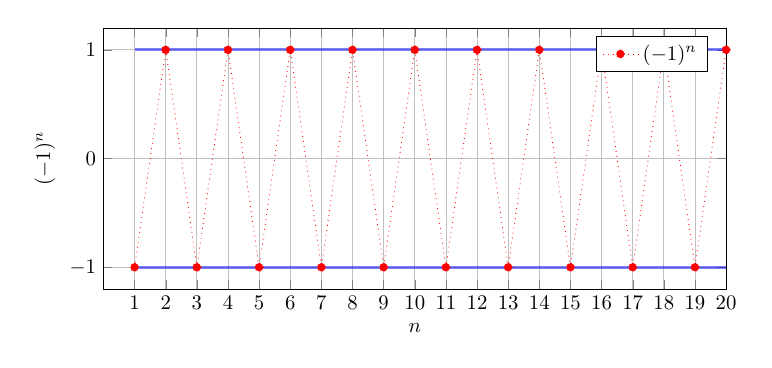
\begin{tikzpicture}[scale=.75]
\begin{axis}[
	xlabel={$n$},
	ylabel={$(-1)^n$},
	ymin=-1.2, ymax=1.2,
	xmin=0, xmax=20,
	xtick={1,2,...,20},
	ytick={-1,0,1},
	grid=major,
	width=\textwidth,
	height=6cm,
	domain=1:20,
	samples=20,
	legend pos=north east,
	]
	\addplot[red, mark=*, dotted, mark options={fill=red}] {(-1)^x};
	\addplot[blue, line width=.5mm, opacity=.5] {1};
	\addplot[blue, line width=.5mm, opacity=.5] {-1};
	\addlegendentry{$(-1)^n$};
\end{axis}
\end{tikzpicture}
\end{center}
\item What is $\textcolor{red}{\pm1}$ for the set $\textcolor{blue}{S=\set{(-1)^n+\frac{1}{n}:n\in\N}}$?
\begin{center}
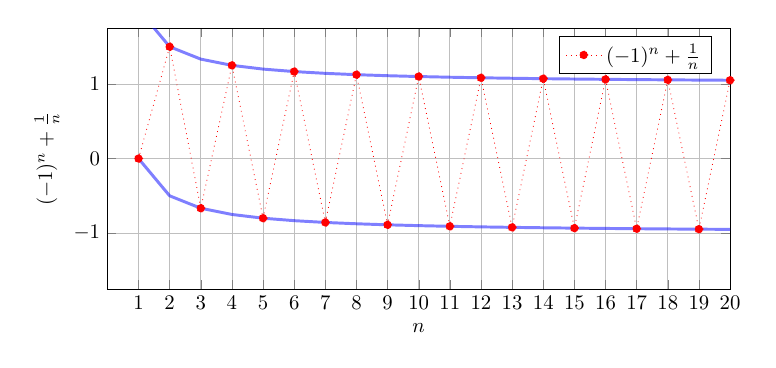
\begin{tikzpicture}[scale=.75]
\begin{axis}[
	xlabel={$n$},
	ylabel={$(-1)^n+\frac{1}{n}$},
	ymin=-1.75, ymax=1.75,
	xmin=0, xmax=20,
	xtick={1,2,...,20},
	ytick={-1,0,1},
	grid=major,
	width=\textwidth,
	height=6cm,
	domain=1:20,
	samples=20,
	legend pos=north east,
	]
	\addplot[red, mark=*, dotted, mark options={fill=red}] {(-1)^x+(1/x)};
	\addplot[blue, line width=.5mm, opacity=.5] {1+(1/x)};
	\addplot[blue, line width=.5mm, opacity=.5] {-1+(1/x)};
	\addlegendentry{$(-1)^n+\frac{1}{n}$};
\end{axis}
\end{tikzpicture}
\end{center}
\end{itemize}
Let $\set{x_n}_{i=1}^\infty$ be a sequence in $\R$. Define \begin{align*}
	s_1 &=\sup\set{x_1,x_2,x_3,\dots}=\sup\set{x_k:k\geq 1}, \\
	s_1 &=\sup\set{x_2,x_3,x_4,\dots}=\sup\set{x_k:k\geq 2}, \\
	&\vdots \\
	s_n &=\sup\set{x_k,x_{k+1},\dots}=\sup\set{x_k:k\geq n}.
\end{align*}
By monotonicity of supremum, $$
s_1\geq s_2\geq\cdots\geq s_n\geq s_{n+1}\geq\cdots.$$
That is, $\set{s_n}_{n=1}^\infty$ be a monotone decreasing sequence. Similarly, for $t_n=\inf\set{x_k,x_{k+1},\dots}=\inf\set{x_k:k\geq n}$, we have a monotone increasing sequence $\set{t_n}_{n=1}^\infty$.
Consider the followings:
\begin{table}[h]
\centering\setstretch{1.25}
\begin{tabular}{c|cc|c||cc}
	\toprule
	\(n\) & \((-1)^n\) & \(\frac{1}{n}\) & \(x_n=(-1)^n + \frac{1}{n}\) & $\sup\set{x_k:k\geq n}$ & $\inf\set{x_k:k\geq n}$ \\
	\midrule
	1  & \(-1\)   & \(1\)       & \(0\) & 1.5 & $-1$ \\
	2  & \(1\)    & \(\tfrac{1}{2}=0.5\)  & \(\tfrac{3}{2}=1.5\) & 1.5 & $-1$   \\
	3  & \(-1\)   & \(\tfrac{1}{3}\approx 0.33\)  & \(-\tfrac{2}{3}\approx -0.67\) & 1.25 & $-1$  \\
	4  & \(1\)    & \(\tfrac{1}{4}=0.25\)  & \(\tfrac{5}{4}=1.25\) & 1.25 & $-1$   \\
	5  & \(-1\)   & \(\tfrac{1}{5}=0.2\)  & \(-\tfrac{4}{5}=-0.8\) & 1.17 & $-1$  \\
	6  & \(1\)    & \(\tfrac{1}{6}\approx 0.17\)  & \(\tfrac{7}{6}\approx 1.17\) & 1.17 & $-1$   \\
	7  & \(-1\)   & \(\tfrac{1}{7}\approx 0.14\)  & \(-\tfrac{6}{7}\approx -0.86\) & 1.125 & $-1$  \\
	8  & \(1\)    & \(\tfrac{1}{8}=0.125\)  & \(\tfrac{9}{8}=1.125\) & 1.125 & $-1$   \\
	9  & \(-1\)   & \(\tfrac{1}{9}\approx 0.11\)  & \(-\tfrac{8}{9}\approx -0.89\) & 1.1 & $-1$  \\
	10 & \(1\)    & \(\tfrac{1}{10}=0.1\) & \(\tfrac{11}{10}=1.1\) & 1.1 & $-1$ \\
	\bottomrule
\end{tabular}
%\caption{Values of \(\displaystyle a_n = (-1)^n + \frac{1}{n}\) for \(n = 1,2,\dots,10\).}
%\label{tab:sequence-(-1)^n+1/n}
\end{table}

\begin{center}
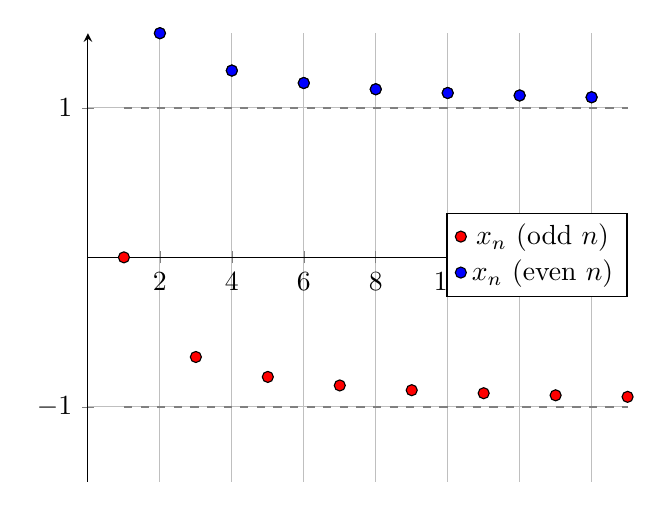
\begin{tikzpicture}
\begin{axis}[
xmin=0, xmax=15,
ymin=-1.5, ymax=1.5,
grid=both,
axis lines=middle,
samples at={1,...,15}, % Plot points for n=1 to 15
clip=false,
legend style={at={(1,.6)}}
]
% Plot the sequence points (even n in blue, odd n in red)
\addplot[
only marks,
mark=*,
mark options={fill=red},
] coordinates {
(1, -1 + 1/1)
(2, 1 + 1/2)
(3, -1 + 1/3)
(4, 1 + 1/4)
(5, -1 + 1/5)
(6, 1 + 1/6)
(7, -1 + 1/7)
(8, 1 + 1/8)
(9, -1 + 1/9)
(10, 1 + 1/10)
(11, -1 + 1/11)
(12, 1 + 1/12)
(13, -1 + 1/13)
(14, 1 + 1/14)
(15, -1 + 1/15)
};
\addlegendentry{\( x_n \) (odd \( n \))}

\addplot[
only marks,
mark=*,
mark options={fill=blue},
] coordinates {
(2, 1 + 1/2)
(4, 1 + 1/4)
(6, 1 + 1/6)
(8, 1 + 1/8)
(10, 1 + 1/10)
(12, 1 + 1/12)
(14, 1 + 1/14)
};
\addlegendentry{\( x_n \) (even \( n \))}

% Draw lim sup and lim inf as dashed lines
\addplot[dashed, gray, thick, no marks] coordinates {(1,1) (15,1)};
\addplot[dashed, gray, thick, no marks] coordinates {(1,-1) (15,-1)};
\end{axis}
\end{tikzpicture}\hfill
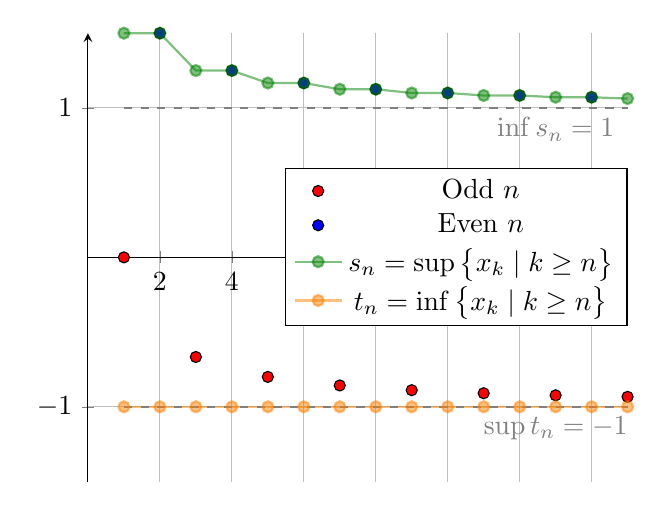
\begin{tikzpicture}
\begin{axis}[
xmin=0, xmax=15,
ymin=-1.5, ymax=1.5,
grid=both,
axis lines=middle,
clip=false,
legend style={at={(1,.7)}}
]

% Original sequence (odd n: red, even n: blue)
\addplot[only marks, mark=*, mark options={fill=red}] coordinates {
	(1, 0)    % x_1 = -1 + 1/1 = 0
	(3, -1 + 1/3)
	(5, -1 + 1/5)
	(7, -1 + 1/7)
	(9, -1 + 1/9)
	(11, -1 + 1/11)
	(13, -1 + 1/13)
	(15, -1 + 1/15)
};
\addlegendentry{Odd \(n\)}

\addplot[only marks, mark=*, mark options={fill=blue}] coordinates {
	(2, 1 + 1/2)
	(4, 1 + 1/4)
	(6, 1 + 1/6)
	(8, 1 + 1/8)
	(10, 1 + 1/10)
	(12, 1 + 1/12)
	(14, 1 + 1/14)
};
\addlegendentry{Even \(n\)}

% Monotone decreasing lim sup sequence (s_n)
\addplot[thick, green!50!black, mark=*, mark size=2pt, opacity=.5] coordinates {
	(1, 1.5)   % s_1 = sup{x_1, x_2, ...} = 1.5
	(2, 1.5)   % s_2 = sup{x_2, x_3, ...} = 1.5
	(3, 1.25)  % s_3 = sup{x_3, x_4, ...} = 1.25
	(4, 1.25)  % s_4 = sup{x_4, x_5, ...} = 1.25
	(5, 1.1667)% s_5 = sup{x_5, x_6, ...} ≈ 1.1667
	(6, 1.1667)
	(7, 1.125) % s_7 = sup{x_7, x_8, ...} = 1.125
	(8, 1.125)
	(9, 1.1)   % s_9 = sup{x_9, x_{10}, ...} = 1.1
	(10, 1.1)
	(11, 1.0833)
	(12, 1.0833)
	(13, 1.0714)
	(14, 1.0714)
	(15, 1.0625)
};
\addlegendentry{\(s_n=\sup\set{x_k\mid k\geq n}\)}

% Monotone increasing lim inf sequence (i_n)
\addplot[thick, orange, mark=*, mark size=2pt, opacity=.5] coordinates {
%	(1, 0)     % i_1 = inf{x_1, x_2, ...} = 0
%	(2, -0.6667) % i_2 = inf{x_2, x_3, ...} ≈ -0.6667
%	(3, -0.6667)
%	(4, -0.8)  % i_4 = inf{x_4, x_5, ...} = -0.8
%	(5, -0.8)
%	(6, -0.8571) % i_6 = inf{x_6, x_7, ...} ≈ -0.8571
%	(7, -0.8571)
%	(8, -0.8889) % i_8 = inf{x_8, x_9, ...} ≈ -0.8889
%	(9, -0.8889)
%	(10, -0.9091) % i_{10} = inf{x_{10}, x_{11}, ...} ≈ -0.9091
%	(11, -0.9091)
%	(12, -0.9231)
%	(13, -0.9231)
%	(14, -0.9333)
%	(15, -0.9333)
(1, -1)
(2, -1)
(3, -1)
(4, -1)
(5, -1)
(6, -1)
(7, -1)
(8, -1)
(9, -1)
(10, -1)
(11, -1)
(12, -1)
(13, -1)
(14, -1)
(15, -1)
};
\addlegendentry{\(t_n=\inf\set{x_k\mid k\geq n}\)}

% Asymptotic limits (dashed lines)
\addplot[dashed, gray, thick] coordinates {(1,1) (15,1)};
\addplot[dashed, gray, thick] coordinates {(1,-1) (15,-1)};
\node[gray, below] at (axis cs:13,1) {\(\inf s_n = 1\)};
\node[gray, below] at (axis cs:13,-1) {\(\sup t_n = -1\)};
\end{axis}
\end{tikzpicture}
\end{center}
\end{observation}
\begin{remark*}
Consider \[
x_n:=(-1)^n+(-1)^n\cdot\frac{1}{n}
\]
\begin{center}
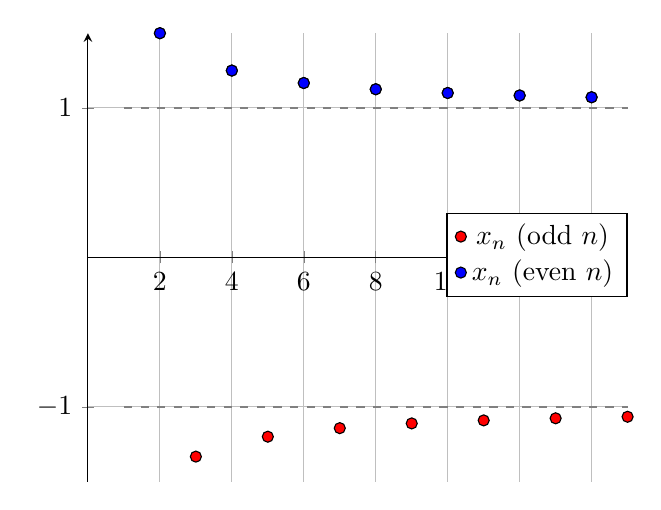
\begin{tikzpicture}
\begin{axis}[
xmin=0, xmax=15,
ymin=-1.5, ymax=1.5,
grid=both,
axis lines=middle,
samples at={1,...,15}, % Plot points for n=1 to 15
clip=false,
legend style={at={(1,.6)}}
]
% Plot the sequence points (even n in blue, odd n in red)
\addplot[
only marks,
mark=*,
mark options={fill=red},
] coordinates {
%	(1, -1 - 1/1)
	(2, 1 + 1/2)
	(3, -1 - 1/3)
	(4, 1 + 1/4)
	(5, -1 - 1/5)
	(6, 1 + 1/6)
	(7, -1 - 1/7)
	(8, 1 + 1/8)
	(9, -1 - 1/9)
	(10, 1 + 1/10)
	(11, -1 - 1/11)
	(12, 1 + 1/12)
	(13, -1 - 1/13)
	(14, 1 + 1/14)
	(15, -1 - 1/15)
};
\addlegendentry{\( x_n \) (odd \( n \))}

\addplot[
only marks,
mark=*,
mark options={fill=blue},
] coordinates {
	(2, 1 + 1/2)
	(4, 1 + 1/4)
	(6, 1 + 1/6)
	(8, 1 + 1/8)
	(10, 1 + 1/10)
	(12, 1 + 1/12)
	(14, 1 + 1/14)
};
\addlegendentry{\( x_n \) (even \( n \))}

% Draw lim sup and lim inf as dashed lines
\addplot[dashed, gray, thick, no marks] coordinates {(1,1) (15,1)};
\addplot[dashed, gray, thick, no marks] coordinates {(1,-1) (15,-1)};
\end{axis}
\end{tikzpicture}\hfill
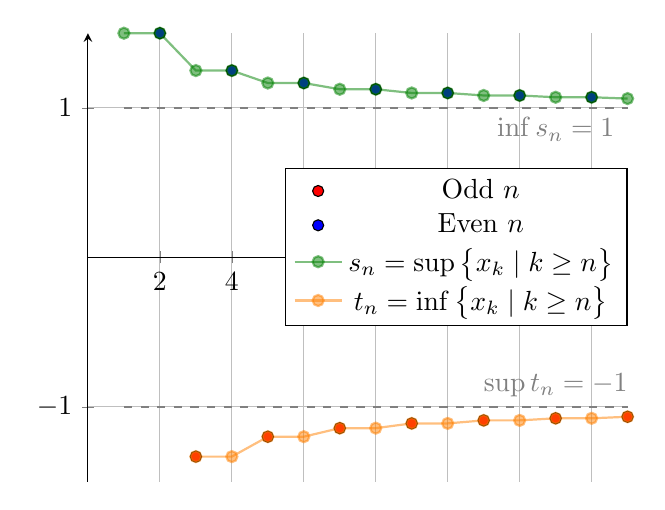
\begin{tikzpicture}
\begin{axis}[
xmin=0, xmax=15,
ymin=-1.5, ymax=1.5,
grid=both,
axis lines=middle,
clip=false,
legend style={at={(1,.7)}}
]

% Original sequence (odd n: red, even n: blue)
\addplot[only marks, mark=*, mark options={fill=red}] coordinates {
%	(1, 0)    % x_1 = -1 + 1/1 = 0
	(3, -1 - 1/3)
	(5, -1 - 1/5)
	(7, -1 - 1/7)
	(9, -1 - 1/9)
	(11, -1 - 1/11)
	(13, -1 - 1/13)
	(15, -1 - 1/15)
};
\addlegendentry{Odd \(n\)}

\addplot[only marks, mark=*, mark options={fill=blue}] coordinates {
	(2, 1 + 1/2)
	(4, 1 + 1/4)
	(6, 1 + 1/6)
	(8, 1 + 1/8)
	(10, 1 + 1/10)
	(12, 1 + 1/12)
	(14, 1 + 1/14)
};
\addlegendentry{Even \(n\)}

% Monotone decreasing lim sup sequence (s_n)
\addplot[thick, green!50!black, mark=*, mark size=2pt, opacity=.5] coordinates {
	(1, 3/2)   % s_1 = sup{x_1, x_2, ...} = 1.5
	(2, 3/2)   % s_2 = sup{x_2, x_3, ...} = 1.5
	(3, 5/4)  % s_3 = sup{x_3, x_4, ...} = 1.25
	(4, 5/4)  % s_4 = sup{x_4, x_5, ...} = 1.25
	(5, 7/6)% s_5 = sup{x_5, x_6, ...} ≈ 1.1667
	(6, 7/6)
	(7, 9/8) % s_7 = sup{x_7, x_8, ...} = 1.125
	(8, 9/8)
	(9, 1.1)   % s_9 = sup{x_9, x_{10}, ...} = 1.1
	(10, 1.1)
	(11, 13/12)
	(12, 13/12)
	(13, 15/14)
	(14, 15/14)
	(15, 17/16)
};
\addlegendentry{\(s_n=\sup\set{x_k\mid k\geq n}\)}

% Monotone increasing lim inf sequence (i_n)
\addplot[thick, orange, mark=*, mark size=2pt, opacity=.5] coordinates {
%(1, -2)
%(2, -2)
(3, -1-1/3)
(4, -1-1/3)
(5, -1-1/5)
(6, -1-1/5)
(7, -1-1/7)
(8, -1-1/7)
(9, -1-1/9)
(10, -1-1/9)
(11, -1-1/11)
(12, -1-1/11)
(13, -1-1/13)
(14, -1-1/13)
(15, -1-1/15)
};
\addlegendentry{\(t_n=\inf\set{x_k\mid k\geq n}\)}

% Asymptotic limits (dashed lines)
\addplot[dashed, gray, thick] coordinates {(1,1) (15,1)};
\addplot[dashed, gray, thick] coordinates {(1,-1) (15,-1)};
\node[gray, below] at (axis cs:13,1) {\(\inf s_n = 1\)};
\node[gray, above] at (axis cs:13,-1) {\(\sup t_n = -1\)};
\end{axis}
\end{tikzpicture}
\end{center}
\end{remark*}
\vfill
\defbox[Limit Superior and Limit Inferior]{\begin{definition*}
Let $\set{x_n}$ be a sequence of real numbers. \st{Suppose that $\set{x_n}$ is bounded.}
\begin{enumerate}[(1)]
	\item The \textbf{limit superior} of $\set{x_n}$, denoted by $\limsup\limits_{n \to \infty} x_n$ (or $\overline{\lim\limits_{n \to \infty}}x_n$) is defined as \[
		\limsup\limits_{n \to \infty} x_n=\lim\limits_{n\to\infty}\left(\sup_{k\geq n}x_k\right):=\inf_{n\in\N}\left(\sup_{k\geq n}x_k\right),
	\] where $\sup_{k\geq n}x_k$ represents the supremum of the subsequence $\set{x_k:k\geq n}$.
	\item The \textbf{limit inferior} of $\set{x_n}$, denoted by $\liminf\limits_{n \to \infty} x_n$ (or $\underline{\lim\limits_{n \to \infty}}x_n$) is defined as \[
	\liminf\limits_{n \to \infty} x_n=\lim\limits_{n\to\infty}\left(\inf_{k\geq n}x_k\right):=\sup_{n\in\N}\left(\inf_{k\geq n}x_k\right),
	\] where $\inf_{k\geq n}x_k$ represents the infimum of the subsequence $\set{x_k:k\geq n}$.
\end{enumerate}
\end{definition*}}
\begin{note}[Extended Real Number Line]
	The \textbf{extended real number line} $\overline{\R}$ is defined as \[
	\overline{\R}:=\R\cup\set{\pm\infty}.
	\] That is, the set of real numbers together with two auxiliary symbols $+\infty,-\infty$ such that \[
	\forall x\in\R,\ -\infty<x<+\infty.
	\]
\end{note}


\thmbox[Bolzano-Weierstrass Theorem]{\begin{theorem*}
	A bounded sequence of real numbers has a convergent subsequence.
\end{theorem*}}


\begin{remark*}
	$\liminf s_n\leq \limsup s_n$
	\begin{proof}
		content...
	\end{proof}
\end{remark*}

\probox{\begin{proposition*}
	$\limsup s_n=\beta\iff\begin{cases}
		\forall\varepsilon>0,\ \exists n_0\in\N\ \text{s.t.}\ n\geq n_0\Rightarrow s_n<\beta+\varepsilon \\
		\forall\varepsilon>0,\ \forall n\in\N\ \exists k\in\N\ \text{s.t.}\ k\geq n\land \beta-\varepsilon< s_k.
	\end{cases}$
\end{proposition*}}

%\begin{tikzpicture}
%	
%	% Create a pgfplots environment
%	\begin{axis}[
%		axis lines=middle,
%		xlabel={$x$},
%		ylabel={$f(x)$},
%		xmin=0, xmax=1.5,
%		ymin=0, ymax=2.25,
%		width=12cm,
%		height=8cm,
%		grid=both,
%		legend style={font=\small},
%		legend pos=north west,
%		samples=100,
%		domain=0:1.5
%		]
%		
%		% Continuous function f(x)
%		\addplot[line width=.5mm, blue, domain=0:1.5] {x^2} 
%		node[pos=0.8, midway, left=2cm] {\textcolor{blue}{$f(x) = x^2$}};
%		
%		% Horizontal dashed line for limit L
%		\addplot[red, dashed, line width=.5mm] coordinates {(0,2) (1.5,2)} 
%		node[pos=0.9, above] {\textcolor{red}{}};
%		\addplot[red, dashed, line width=.5mm] coordinates {({sqrt(2)},0) ({sqrt(2)},2)};
%		
%		% Point p (limit point)
%		\addplot[mark=*, mark options={red}, only marks] coordinates {({sqrt(2)},2)} 
%		node[below] {\textcolor{red}{}};
%		
%		% Sequence points approaching p
%		\addplot[line width = .75mm, mark=*, teal, opacity=0.75] coordinates {(0,0) (.2,{.2^2}) (.4,{.4^2}) (.9,{.9^2}) ({sqrt(2)},2)}
%		node[pos=0.1, below right] {\textcolor{teal}{$\set{x_n,f(x_n)}$}};
%%		
%%		% Annotate sequence x_n -> p
%%		\draw[->, thick, orange] (axis cs:0.8,0) -- (axis cs:1,0) 
%%		node[midway, below] {\textcolor{orange}{$x_n \to p$}};
%%		
%%		% Annotate f(x_n) -> L
%%		\draw[->, thick, orange] (axis cs:0.99,0.9801) -- (axis cs:1,1) 
%%		node[midway, right] {\textcolor{orange}{$f(x_n) \to L$}};
%%		
%%		% Neighborhood of p
%%		\draw[<->, thick, red] (axis cs:0.85,-0.1) -- (axis cs:1.15,-0.1)
%%		node[midway, below] {\textcolor{red}{$\delta$}};
%		
%		% Legend
%%		\legend{
%%			$f(x)$ (continuous),
%%			Limit $L$,
%%			Limit point $p$,
%%			Sequence points $\{x_n\}$
%%		}
%		
%	\end{axis}
%	
%\end{tikzpicture}


\vfill

\begin{thebibliography}{9}
	\bibitem{advanced_calc_e}
	수학의 즐거움, Enjoying Math. ``수학 공부, 기초부터 대학원 수학까지, 10. 해석학 개론 (e) 엡실론-델타와 수열의 수렴성'' YouTube Video, 25:57. Published 
	September 29, 2019. URL: \url{https://youtu.be/2Ml3G_Duffk?si=qo-CVgW3Ukd4ADRL}.
	\bibitem{advanced_calc_f}
	수학의 즐거움, Enjoying Math. ``수학 공부, 기초부터 대학원 수학까지, 11. 해석학 개론 (f) MCT and NIP'' YouTube Video, 20:17. Published 
	October 1, 2019. URL: \url{https://youtu.be/YdnBQaY5eDk?si=BNe0Ue4iq2P9Fxsd}.
	\bibitem{advanced_calc_g}
	수학의 즐거움, Enjoying Math. ``수학 공부, 기초부터 대학원 수학까지, 12. 해석학 개론 (g) Limsup, Liminf'' YouTube Video, 34:31. Published 
	October 2, 2019. URL: \url{https://youtu.be/4Q1cm3VQPUE?si=phAhKwnOxdnRAiRR}.
\end{thebibliography}

\newpage
\appendix
%\section{Application of Monotone Convergence Theorem (Euler Number $e$)}
%\paragraph{Problem.} Prove that \[
%\lim\limits_{n\to\infty}\left(1+\frac{1}{n}\right)^n
%\] exists.
%\begin{proof}[\sol]
%Recall that Binomial Theorem: \[
%(x+y)^n=\sum_{k=0}^{n}\binom{n}{k}x^ky^{n-k}.
%\]
%\end{proof}
\section{Equivalent Statements of the Least Upper Bound Property}
\begin{align*}
\text{Least Upper Bound Property}&\iff\text{Monotone Convergence Theorem}\\
&\iff\text{Nested Interval Property}
\end{align*}

\thmbox[]{\begin{theorem*}
Monotone Convergence Theorem $\iff$ Nested Interval Property
\end{theorem*}}
\begin{proof}
\begin{enumerate}
\item[($\Rightarrow$)] See \hyperlink{nip}{\textbf{Nested Interval Property}}.
\item[($\Leftarrow$)] TBA
%Let $\set{a_n}_{n=1}^\infty$ is a bounded monotone sequence.
%\begin{enumerate}[]
%	\item
%	(Case 1) Let $\set{a_n}$ is monotone increasing. Since $\set{a_n}$ is bounded above, let $M$ be an upper bound. Construct a nested interval sequence: \[
%	\intcc{a_n,M}.
%	\] Clearly, $a_n\leq M$ and $\intcc{a_{n+1},M}\subseteq\intcc{a_n,M}$. By NIP, \[
%	\exists L\in\R\ \text{such that}\ L\in\intcc{a_n,M}\ \text{for all}\ n\in\N.
%	\]
%\end{enumerate}
\end{enumerate}
\end{proof}
\thmbox[]{\begin{theorem*}
Least Upper Bound Property $\iff$ Monotone Convergence Theorem
\end{theorem*}}
\begin{proof}
\begin{enumerate}
\item[($\Rightarrow$)] See \hyperlink{mct}{\textbf{Monotone Convergence Theorem}}.
\item[($\Leftarrow$)] TBA
\end{enumerate}
\end{proof}
\end{document}
